\chapter{Experimentations}
\chaptermark{Experimentations}
\label{chap:experimentations}
\graphicspath{{./chapters/6-experiments/figs/}}


% \modif{TODO add total number of annotated elements for each category and report the diversity of style, format, publishing from the IJDAR paper}

% Abstract-----------------------------------------------------
With the analysis and processing of data comes the need of the output results evaluation.
Traditionally, this evaluation is made by validating the results of an algorithm with a ground truth that represents what an ideal output should be\cite{pascal-voc-2012, smeaton2006evaluation, griffinHolubPerona}.
Ideally, such a ground truth is made publicly available so anyone can challenge his own algorithm to the community \cite{lamiroy:inria-00537035}.
This can be applied to any kind of results from image segmentation to classification or information retrieval.
In this chapter we present the dataset and ground truth we provide to evaluate comic book image related works.
We describe the metrics we use to evaluate our each contribution (sequential, independent and knowledge-driven) and finally compare them in the global evaluation section.
% compare our work to previous approaches from the literature.

% We evaluate the contributions of the thesis at different levels.
% We first evaluate the sequential, independent and knowledge-driven approaches separately and then we compare them in the global evaluation section.


% \section{Introduction} % (fold)
% \label{sec:ex:introduction}

% TODO

% section introduction (end)

\section{Dataset and ground truth construction} % (fold)
\label{sec:dataset_and_ground_truth_construction}

Being in need of comic books material and an associated ground truth to evaluate our work, we noticed that there is not such dataset publicly available for scientific purpose. 
Therefore, we decided to gather the first publicly available comic books dataset in association with several comic books authors and publishers and to build up the corresponding ground truth according to document analysis and understanding concerns.% which are image segmentation and semantic analysis.
The comic book images were selected to cover the huge diversity of comic styles with the agreement of the consenting authors and publishers that had the objective to foster innovation in this domain trough academic research (Figure~\ref{fig:ex:comics_diversity}).

%%%%%%%%%%%%%%%%%%%%%%%%%%%%%%%%%%%%%%%%%%%%%%%%%%
\begin{figure}[ht]  %trim=l b r t  width=0.5\textwidth,
   \centering
  \includegraphics[trim= 4px 0px 0px 0px, clip, width=230px]{comics_diversity.png}
  \caption[Examples of comic panels that reflect the diversity of comic books of the dataset]{Examples of comic panels that reflect the diversity of comic books of the dataset.}
  \label{fig:ex:comics_diversity}
 \end{figure}

%%%%%%%%%%%%%%%%%%%%%%%%%%%%%%%%%%%%%%%%%%%%%%%%%%

It took almost one year to define which type of comics are the most interesting for researchers, meet and convince comic book authors and publishers, get copyright authorizations for the scientific community, develop a specific annotation tool and finally to hire people to do the ground truth (manual task).

A selection of hundred comic pages were annotated in one day by twenty volunteers affiliated to the L3i lab.
In order to provide a common basis for evaluating research work, the ground truth have been published in 2013~\cite{Guerin2013} and made available to the scientific community through a dedicated website\footnote{\url{http://ebdtheque.univ-lr.fr}}.
It has been enriched in 2014 by adding semantic information to the already annotated elements.

The content of the dataset and its terms of use, the ground truth construction protocol and its quality assessment are detailed in the four next sub sections.



% \section{Structure and indexation}
% \label{sec:gt:structure_indexation}
\subsection{Dataset description} % (fold)
\label{sec:dataset_description}

% section dataset_description (end)

Scott McCloud defined comics as ``juxtaposed pictorial and other images in deliberate sequence, intended to convey information and/or to produce an aesthetic response in the viewer''~\cite{mccloud1994understanding}.
This definition is intentionally broad enough to encompass the spectrum of the majority of works produced so far.
The dataset composition should reflects this heterogeneity to give everyone the opportunity
to compare its algorithms to a globally representative dataset of the comics world.
We contacted authors with different comic styles and have selected a corpus of one hundred images, representing single or double comics page.

The images were partly processed by the French company A3DNum\footnote{\url{http://www.a3dnum.fr}} which was commissioned to digitize 14 albums.
Among all the files, scanned at a resolution of 300 dots per inch and encoded in uncompressed Portable Network Graphic (PNG) format, we used 46 pages to integrate the eBDtheque corpus.
The remaining 54 images were selected from webcomics, public domain comics\footnote{\url{http://digitalcomicmuseum.com}} and unpublished artwork with different styles from 72 to 300 dots per inch.
We encoded all the images of the eBDtheque dataset in Joint Photographic Experts Group (JPEG) format with a lossy compression to facilitate file exchange.
%, the non compressed images are available on request.

Hereafter we describe the characteristics of the selected pages and their content.


\paragraph{Albums} % (fold)
 \label{par:albums}
 published between 1905 and 2012.
 29 pages were published before 1953 and 71 after 2000.
 Quality paper, colour saturation and textures related to printing technique changes can vary a lot from one image to another.
 The artworks are mainly from France (81\%), United States (13\%) and Japan (6\%).
 Their styles varies from classical Franco-Belgium ``bandes dessinées'' to Japanese manga through webcomic and American comics.

 % paragraph albums (end)

\paragraph{Pages} % (fold)
\label{par:pages}
 themselves have very diverse characteristics.
Among all, 72 are printed in colours and according to the authors and periods, there are a majority of the tint areas, watercolours and hand-coloured areas.
Among the remaining 28, 16 have are greyscale and 12 are simply black and white.
One album has two versions of each page, one in colour and the other one in black and white.
We have integrated an examples of each of them in order to allow performance comparison of algorithms on the same graphic style by using colour information or not.
Five of the 100 images are double page, others are single page and 20\% are not A4 format.
% We therefore, strictly speaking, 105 and 100 pages not in our database, each with a distinct structure
% paragraph pages (end)

\paragraph{Panels} % (fold)
\label{par:panels}
 contained in the pages are of various shapes.
Although most of them are bounded by a black line, a significant proportion has at least one part of the panel which is indistinguishable from the background of the page (frame less panel).
Two pages consist only of frame less panels, the visual delimitation uses background contrast difference between the panel and image.
Nine images contain overlapping panels, twelve contain only panels without border and several has panels connected by an straddle object.

% paragraph panels (end)

\paragraph{Balloons} % (fold)
\label{par:balloons}
 also contain a great diversity.
Some of them are completely surrounded by a black stroke, some partially and others not at all.
They have a bright background with a rectangular, oval or non geometric shape with ``smooth'', ``wavy'' or ``spiky'' contour in general.
Most of them has a tail pointing towards the speaker, but some do not.
There is text without any surrounding balloons on 33 images of the corpus.
% and 8 of them simply contain no bubble.

% paragraph balloons (end)

\paragraph{Text} % (fold)
\label{par:text}
 is either typewritten (61\% of the image) or handwritten, mainly upper-case.
The text lines contains 12 elements in average (Figure~\ref{fig:ex:textline_lenth_distribution}) and there are more than hundred text lines that are composed by only one letter corresponding to punctuation or single letter words such as ``I'' or ``A''; this is a particularity of comics.

Most pages are from French artworks, where the text is written in French.
Only 13 pages contain English text and 6 images are in Japanese.
Onomatopoeia appears in 18 pages.

    %%%%%%%%%%%%%%%%%%%%%%%%%%%%%%%%%%%%%%%%%%%%%%%%%%%%%%%%
    \begin{figure}[ht]%trim=l b r t  width=0.5\textwidth,  
      \centering
      \includegraphics[trim= 0px 5px 65px 5px, clip, width=0.85\textwidth]{number_of_letter_per_textline.png}
      \caption[Distribution of the number of elements per text lines]{Distribution of the number of elements per text lines.
      }
      \label{fig:ex:textline_lenth_distribution}
    \end{figure}  
    %%%%%%%%%%%%%%%%%%%%%%%%%%%%%%%%%%%%%%%%%%%%%%%%%%%%%%%%

% paragraph text (end)

\paragraph{Comic characters} % (fold)
\label{par:comic_characters}
or protagonist are specific to each album.
They all have eye, harm and leg but at least 50\% are not humanoid, depending on the interpretation.
% paragraph comic_characters (end)

\subsection{Terms of use} % (fold)
\label{sub:term_of_use}
We obtain the minimum rights for sharing and publishing image material from the right holders but we had to make sure the user accept it before using the data.
In collaboration with the intellectual property department of the University of La Rochelle, we established the following:

\textit{In order to use this database, you must firstly agree to the terms.
You may not use the database if you don't accept the terms.
The use of this database is limited to scientific and non-commercial purpose only, in the computer science domain.
For instance, you are allowed to split the images, through the use of segmentation algorithms.
You can also use pieces of this database to illustrate your research in publications and presentations.
Any other use case must be validated by our service.
If you do agree to be bound by all of these Terms of Use, please fill and email the request form and then use the login and password provided to download the selected version below.}

The concerned request form requires the identity, affiliation, address and intended use of the person who wishes to use data.

% subsection term_of_use (end)

\subsection{Ground truth construction} % (fold)
\label{sec:ground_truth_construction}

The ground truth has been defined in accordance to existing formalism in order to fulfil the needs of a large amount of researchers related to comics material.
It integrates low and high level information such as spatial position of the elements in the image, their semantic links and also bibliographic information.

In order to cover a wide range of possible research matters, it has been decided to extract three different type of objects from the corpus: text lines, balloons and panels.
We decided to do this first ground truth by drawing horizontal bounding boxes as close as possible from the feature and including all its pixels.
% in order to proceed a maximum of pages in the allowed time. 
We chose this level of granularity in order to limit the subjectiveness of the person making the annotation.

The comics art is extremely heterogeneous and our dataset voluntarily integrates albums that can be classified as
unconventional.
This leaves room for interpretation on the form which increase annotation variations by different people and decrease the uniformity of the ground truth.
This precision level is used in several, widely used datasets~\cite{pascal-voc-2012, yao2007introduction}.
%{\color{blue}This groundtruthing level is also used for well known dataset widely used~\cite{pascal-voc-2012, yao2007introduction}.}

Hereafter we detail the two levels of annotation (visual and semantic) that form the ground truth and how they are indexed in a file.
The combination of visual and semantic annotation provides the advantage of making this ground truth relevant for document analysis and semantic evaluation which are both part of the comics understanding process.

% each element to annotate and the protocol to follow.
% follows specific guidelines according to the rules below:

\subsubsection{Visual annotation} % (fold)
\label{sub:visual_annotation}
The first annotation consist in defining the spacial region where elements are located in the image.
We describe hare how the visual annotation have been performed for the panels, balloons, texts and comic characters.

% subsection visual_annotation (end)
\paragraph{Panels} % (fold)
\label{par:panels}
The frame or panels are defined as an image area, generally rectangular, representing a single scene in the story. 
There is always at least one panel per page, the entire page region can be used as panel if necessary.
When a panel has a black border, the bounding box is placed as close as possible to its frame.
Sometimes, images have not been scanned perfectly horizontally, it is then impossible to have an horizontal bounding box sticking exactly to the border.
When the panel border is partially absent or suggested by the neighbourhood, the bounding box just defines the content of the panel.
In all cases, the other elements (balloon, text, drawings) extending from the frame are truncated (Figure~\ref{fig:gt:segPanel}).

%%%%%%%%%%%%%%%%%%%%%%%%%%%%%%%%%%%%%%%%%%%%%%%%%%%%%%%%%
\begin{figure}[h!]
\begin{center}
\includegraphics[width=0.8\textwidth]{segPanel.png}
\caption[Panel annotation]{Example of three panel annotations. The bounding box (transparent red) is defined without taking into account of non panel elements in all cases.}
\label{fig:gt:segPanel}
\end{center}
\end{figure}
%%%%%%%%%%%%%%%%%%%%%%%%%%%%%%%%%%%%%%%%%%%%%%%%%%%%%%%%%

%They can be frame-less, in that case the bounding box will be set according to the contained drawings, see Fig. \ref{fig:segmentation}c. %, ignoring text and overlapping features.
%In both cases, text and overlapping features are ignored.
%There is necessarily at least one panel in a page. 
% paragraph panels (end)

% The panel reading order is also annotated in a metadata called \texttt{rank}, it is in integer  between $1$ and $n$ which is increased incrementally from the first to the last panel $n$ in an image.%, le premier de la séquence prenant la valeur $1$ et le dernier la valeur $n$ pour une page contenant $n$ cases.

\paragraph{Balloons} % (fold)
\label{par:balloons}
We define a balloon (phylactery or bubble) as the region of an image including one or several lines of text, graphically defined by an identifiable physical boundary or suggested by the presence of an arrow pointing to the speaker (the tail).
Although rare, empty balloons (not containing lines of text) are also annotated if they are clearly identifiable by their shape or
the tail representation.
Pixel level annotation follows the contour of the balloon (Figure~\ref{fig:gt:segBalloons}c), while bounding box annotation does not consider the contour of phylactery and truncates the tail.
Sometimes it crosses the entire panel and generates an unrepresentative position of the desired balloon (Figure~\ref{fig:gt:segBalloons}a).
When the balloon is not closed (e.g. open contour) the annotated contour has to stick as close as possible to the contained text (Figure~\ref{fig:gt:segBalloons}b).
Note, the first version of the ground truth (2013) have been defined at bounding box level ignoring the tail and the second version (2014) at pixel level following the contour variations and the tail region.

%%%%%%%%%%%%%%%%%%%%%%%%%%%%%%%%%%%%%%%%%%%%%%ù
\begin{figure}[h!]
\begin{center}
\begin{tabular}{ccc}
a) \includegraphics[width=80px]{segBalloon1.png} 
& 
b) \includegraphics[width=80px]{segBalloon2.png}
&
c) \includegraphics[width=80px]{segBalloon3.png}
\end{tabular}
\caption[Speech balloon contour annotation]{Example of balloon clipping: a) using bounding box excluding the tail, b) bounding box of non closed balloon, c) pixel level contour annotation.} 
\label{fig:gt:segBalloons}
\end{center}
\end{figure}
%%%%%%%%%%%%%%%%%%%%%%%%%%%%%%%%%%%%%%%%%%%%%%ù

% paragraph balloons (end)

\paragraph{Text lines} % (fold)
\label{par:text_lines}
The text lines are defined as a sequence of text characters aligned in the same direction (Figure~\ref{fig:gt:segLines}a).
This definition encompasses both speech texts and narrative text, often located inside balloon, onomatopoeia (graphic sound) that are written or drawn directly in the panel without particular container.
%The text of the latter, although they are occasionally parallel to the edges of the box is still clipped by a horizontal bounding box for consistency across the ground truth.
Comics are static graphics, the expression of emotions of a comic character is the joint action of drawing and text, sometimes in the form of a single punctuation symbol.
For instance, an exclamation mark for surprise or a question mark for a misunderstanding.
These isolated symbols convey information and are segmented as text line as well (Figure~\ref{fig:gt:segLines}b).
Similarly, we have chosen to include in this category the illustrative text, such as a road sign or storefront (Figure~\ref{fig:gt:segLines}c).
Although at the boundary between text and graphic, these elements are still invariably read by the reader and their annotation is potentially interesting for multiple purposes, including story and scene analysis.

%%%%%%%%%%%%%%%%%%%%%%%%%%%%%%%%%%%%%%%%%%%%%%ù
\begin{figure}[h!]
\begin{center}
\begin{tabular}{ccc}
a) \includegraphics[width=80px]{segLine1.png} 
& 
b) \includegraphics[width=80px]{segLine2.png}
&
c) \includegraphics[width=80px]{segLine3.png}
\end{tabular}
\caption[Text line location annotation]{Different examples of text line position annotation: a) a classical text line in a speech balloon, b) a unique symbol, c) illustrative text, non horizontal.} 
\label{fig:segLines}
\end{center}
\end{figure}
%%%%%%%%%%%%%%%%%%%%%%%%%%%%%%%%%%%%%%%%%%%%%%ù

% paragraph text_lines (end)

\paragraph{Comic characters} % (fold)
\label{par:comic_characters}
The comic characters position have been included in the second version of the ground truth only (2014).
The concept of ``character'' may have different interpretations when used for comics and must be specified.
Characters in a comic have not necessarily a human-like, or even living beings appearance.
Even so, it would be appropriate to annotate every human being appearing in a box while some are nothing but a part of the scenery.
Therefore, we have chosen to limit the annotation to the comic characters that emits at least one speech balloon in the album (minimal impact in the story).
Their bounding box has been defined to maximize the region occupied by the comic character inside the box region.
Therefore, some parts of the character such as arms or legs, are clipped sometimes (Figure~\ref{fig:gt:segCharater}).

%%%%%%%%%%%%%%%%%%%%%%%%%%%%%%%%%%%%%%%%%%%%%%
\begin{figure}[h!]
\begin{center}
\includegraphics[width=0.75\textwidth]{segCharacter.png}
\caption[Comic character position annotation]{Example of comic character annotation: sniper's arms are not included in the bounding box in order to maximize the region occupied by the sniper in its bounding box. The two snipers and the two characters in the car are annotated because they emit a speech balloon in a different panel.}
\label{fig:gt:segCharacter}
\end{center}
\end{figure}
%%%%%%%%%%%%%%%%%%%%%%%%%%%%%%%%%%%%%%%%%%%%%%

% paragraph comic_characters (end)


% section ground_truth_construction (end)

\subsubsection{Semantic annotation} % (fold)
\label{sub:gt:semantic_annotation}
This second level of annotation complete each spacial region with additional information about its semantic.
Also, the image itself is annotated with extra information about its origin (e.g. album, collection, author, publisher).
%Once segmented, each object is annotated with a set of predefined metadata as follows. 

TODO describe metadata attribute \emph{idBalloon} in Line elements and \emph{idCharacter} in Character element

\paragraph{Images}
The image, often assimilated as pages, has been annotated with bibliographical information, so that anyone using this ground truth is free to get is own paper copy of the comic books for extra uses.
The first annotation is the page number (\texttt{{pageNumber}}) then the comic book title, from which the page has been picked up, and its release date (\texttt{{albumTitle, releaseDate}}), the series it belongs to (\texttt{{collectionTitle}}), the authors and editor names (\texttt{{writerName, drawerName, editorName}}) and, finally, the website and/or ISBN (\texttt{{website, ISBN}}).
The album title is not mandatory for webcomics.
Structural information about the page content has been added as well, such as resolution (\texttt{{resolution}}), reading direction (\texttt{{readingDirection}}), main language of the text (\texttt{{language}}) and single or double page information (\texttt{{doublePage}}).
% These annotation are stored in a tag named \texttt{{Pages}}.

\paragraph{Panels} 
The panes are annotated with a \texttt{{rank}} metadata which stand for its position in the reading sequence. 
The first panel to be read on a given page has its rank property set to 1, while the last one is set to \textit{n}, where \textit{n} is the number of panels in the page.

\paragraph{Balloons}
Balloons are also annotated with a \texttt{{rank}} property that defines their reading order relatively to the image because balloons are not always included in panels.
%, their rank is set according to the page as a whole. 
For a page containing $m$ balloons, the first balloon's rank will be 1 and the last will be $m$.
%Moreover, two additional metadata are given. 
A second information concerns the \texttt{{shape}} of the balloon.
This feature conveys an information about how the contained text is spoken (tone).
The type of \texttt{{shape}} is given from the following list \{\texttt{smooth, wavy, spiky, suggested}\} as pictured in figure~\ref{fig:gt:balloonShape}.
Finally, the tail tip position (extremity) and its pointing direction have been added into the second version of the ground truth.
There are given through the \texttt{{tailTip}} and \texttt{{tailDirection}} properties.
The possible values of the direction are reduced to the eight cardinal directions plus a ninth additional value for the lack of tail: \{\texttt{N, NE, E, SE, S, SW, W, NW, none}\}.
In the second version of the ground truth (2014), we added the identifier of the comic character which is emitting the balloon \texttt{{idCharacter}}. 

%%%%%%%%%%%%%%%%%%%%%%%%%%%%%%%%%%%%%%%%%%%%%%%%%%%
\begin{figure}[h!]
\begin{center}
\includegraphics[width=0.65\textwidth]{balloonShape.png}
\caption[Balloon shapes]{Les différents types de contour de bulle, de gauche à droite et de haut en bas : nuage, hérissé, suggéré, rectangle, ovale.}
\label{fig:gt:balloonShape}
\end{center}
\end{figure}
%%%%%%%%%%%%%%%%%%%%%%%%%%%%%%%%%%%%%%%%%%%%%%%%%%%

\paragraph{Text lines}
The text lines are associated with their transcription and the identifier of the corresponding balloon is added in \texttt{{idBalloon}} if the text line is included in a balloon.

\paragraph{Comic characters} % (fold)
\label{par:comic_characters}
The comic character are identified by \texttt{{idCharacter}} in order to be easily referred.

% paragraph comic_characters (end)

% \paragraph{Speaking character and speech balloon} % (fold)
% \label{par:speaking_character_and_speech_balloon}
% In the second version of the ground truth, we added a new type of relation which is between regions.
%  balloons and comic characters regions that are related in the story (balloon spoken by a character).
% The information is stored in a structure called \texttt{{LinkSBSC}} that consist a pair of identifier \texttt{{idBalloon}} and \texttt{{idCharacter}}.
% paragraph speaking_character_and_speech_balloon (end)


%%%%%%%%%%%%%%%%%%%%%%%%%%%%%%%%%%%%%%%%%%%
% \begin{figure}
% \begin{center}
% \includegraphics[width=0.45\textwidth]{balloons_shape3.png}
% \caption{Different speech balloon shapes. Top-down, from left to right: cloud, peak, suggested, rectangular and oval.}
% \label{fig:balloons_shape}
% \end{center}
% \end{figure}
%%%%%%%%%%%%%%%%%%%%%%%%%%%%%%%%%%%%%%%%%%%

% subsection semantic_annotation (end)

\subsubsection{File structure} % (fold)
\label{sub:file_structure}

The ground truth file structure have been thought according to existing comics related formalism such as Comics Markup Language (ComicsML)~\cite{McIntosh2011}, Comic Book Markup Language (CBML)~\cite{Walsh2012a}, Periodical Comics\footnote{\url{http://www.w3.org/wiki/WebSchemas/PeriodicalsComics}}, A Comics Ontology~\cite{Rissen2012}, Advanced Comic Book Format (ACBF)\footnote{\url{https://launchpad.net/acbf}} and the Grand Comics Database (GCD)\footnote{\url{http://www.comics.org}}.
See the Ph.D. thesis of Gu{\'e}rin~\cite{phdthesisGuerin14} for an extended review.

As we wanted to keep the ground truth file system simple and easy to share, visual and semantic annotations about a given page are gathered in a single full-text file following the specifications of Scalable Vector Graphics (SVG). 
Besides being an open-standard developed by the World Wide Web Consortium (W3C) since 1999, the SVG format fulfils two essential needs for this database.

First, using a recent Internet browser or your favourite image viewer, it provides a simple, fast and elegant way to display the visual annotation of any desired object over a comic book page using layers.
No need to install software such as Matlab, Adobe Illustrator or equivalent open source to visualize the ground truth information.

It is XML-based vector image format that allows to display an animate the annotated region, stored as polygon object in the SVG file, as desired using the Cascading Style Sheets (CSS) properties (Figure~\ref{fig:gt:svgImage}). 

%%%%%%%%%%%%%%%%%%%%%%%%%%%%%%%%%%%%%%%%%%%%%%%%%

\begin{figure}[h!]
\begin{center}
\begin{tabular}{ccc}
a) \includegraphics[width=100px]{svgPanel.png} 
& 
b) \includegraphics[width=100px]{svgBalloon.png}
&
c) \includegraphics[width=100px]{svgTextlines.png}
\end{tabular}
\caption[Annotation rendering in a browser]{Example of rendering for each class of element. For example, red for panels (a), cyan for balloons (b) and green for text (c). The opacity is set to 50\% to allow seeing the corresponding image by transparency.} 
\label{fig:gt:svgImage}
\end{center}
\end{figure}
%%%%%%%%%%%%%%%%%%%%%%%%%%%%%%%%%%%%%%%%%%%%%%%%%%

Each layer can be displayed or not in order to enhance the clearness of the annotations when browsing the database.
Secondly, SVG being a XLM-based language, it makes the integration of semantic annotation very easy via the use of the predefined \texttt{metadata} element.

One ground truth file contains the complete description of one comics image. 
There is no hierarchical link between pages from a same comic book. 
Following the basic XML encoding information, a SVG file starts with a root \texttt{<svg>} element containing the title of the document, \texttt{<title>}, and five \texttt{<svg>} children with different class attributes.
These contain annotations collected on five types of elements which are the page, panels, balloons, text lines and comic characters.
The type of element in a tag is specified by its \texttt{class} attribute.
The first tag, \texttt{class = ``Page''} contains description on the image and has two daughters.
The first one, \texttt{image} has several attributes which specifies a link to the image file in the dataset \texttt{xlink: href} and two specifying the \texttt{width} and \texttt{height} of the image.
The second, \texttt{metadata}, contains bibliographic information about the album and page properties described in \ref{sub:gt:semantic_annotation}.
%A SVG file begins with information about the XML version and encoding system and then a root \texttt{<svg>} element containing the title of the document \texttt{<title>} and four others \texttt{<svg>} elements with different class attributes. % that describe the page, the panels, the text lines and the text areas the entire set of annotations for the attached page.
%The annotations are the same for all the \texttt{<svg>} nodes, each of them describing one kind of element (e.g. panel, balloon) according to its {\tt class} attribute. 
%The first \texttt{<svg>} element, \texttt{<svg class=``Page''>}, has two children.
%The first one is \texttt{<image>} and contains a link to the corresponding image file and the size it has to be displayed.
%The next child is a \texttt{<metadata>} element containing the bibliographical information described in \ref{sub:gt:semantic_annotation}.
The four following \texttt{<svg>} siblings, \texttt{<svg class=``Panel''>}, \texttt{<svg class=``Balloon''>}, \texttt{<svg class=``Line''>} and \texttt{<svg class=``Character''>} respectively contain the annotations about panels, balloons, text lines and comic characters. 
They all contain SVG \texttt{<polygon>} elements with a list of five or more points in a \texttt{point} attribute that define the position of the bounding box corners or the pixel-level contour. %four corners position coordinates of a bounding box. 
Note that the last point is always equal the first one to ``close'' the polygon according to the SVG specifications. 
Those points are used by the viewer to draw polygons with the corresponding CSS style. 
Each \texttt{<polygon>} has a \texttt{<metadata>} child to store information on the corresponding polygon, according to the attributes list described in \ref{sub:gt:semantic_annotation}.

An example of ground truth file is given figure~\ref{list:svg}.% présente un exemple du contenu de l'un de ces fichiers.

\begin{lstlisting}[language=XML, frame=single, caption=Sample of SVG file from the eBDtheque ground truth, captionpos=b, label=list:svg]
<?xml version="1.0" encoding="UTF-8" standalone="no"?>
<svg>
  <title>CYB_BUBBLEGOM_T01_005</title>
  <svg class="Page">
    <image 
      x="0" 
      y="0" 
      width="750" 
      height="1060" 
      href="CYB_BUBBLEGOM_T01_005.jpg"
    />
    <metadata 
      collectionTitle="Bubblegom_Gom"
      editorName="Studio_Cyborga" 
      doublePage="false"
      website="http://bubblegom.over-blog.com"
      albumTitle="La_Legende_des_Yaouanks"
      drawerName="Cyborg_07"
      language="french"
      resolution="300"
      ISBN="979-10-90655-01-0"
      readingDirection="leftToRight" 
      writerName="Cyborg_07"
      releaseDate="2009"
      pageNumber="5"
    />
  </svg>
  <svg class="Panel">
    <polygon points="53,95 268,95 268,292 53,292 53,95">
      <metadata 
        idPanel="P01"
        rank="1"
      />
    </polygon>
    ...
  </svg>
  <svg class="Balloon">
    <polygon points="61,103 143,103 143,172 61,172 61,103">
      <metadata
        idBalloon="B01" 
        shape="smooth"
        tailTaip="153,167"
        tailDirection="SE" 
        rank="1"
      />
    </polygon>
    ...
  </svg>
  <svg class="Line">
    <polygon points="373,121 432,121 432,132 373,132 373,121">
      <metadata 
        idLine="L01"
        idBalloon="B01"
      >
        LIKE YOU.
      </metadata>
    </polygon>
    ...
  </svg>
  <svg class="Character">
    <polygon points="84,153 261,153 261,298 84,298 84,153"/>
      <metadata idCharacter="C01"/>
    ...
  </svg>
  <svg class="LinkSBSC">
    <polygon points="34,234 56,235 79,340 79,339 34,234"/>
      <metadata 
        idLinkSBSC="LSBSC01"
        idBalloon="B01"
        idCharacter="C01"
      />
    ...
  </svg>
</svg>
\end{lstlisting}

%{\bf Add SVG code figure here?} Arnaud suggested it too but, we don't have room and it will be ugly...

%
%\begin{lstlisting}
%<svg>
%</svg>
%\end{lstlisting}

%{\color{red}short file as an illustration?}

% \begin{figure}
% \begin{center}
% \begin{tabular}{ccc}
% \includegraphics[width=0.14\textwidth]{fig/bbg_panel2.png} & 
% \includegraphics[width=0.14\textwidth]{fig/bbg_balloon2.png} &
% \includegraphics[width=0.14\textwidth]{fig/bbg_textlines2.png}
% %\includegraphics[width=0.20\textwidth]{fig/bbg_all.png} &
% \end{tabular}
% \caption{Left-to-right: segmentation of a panel, a speech balloon and text lines. Credits: \cite{Bubble09}}
% \label{fig:css}
% \end{center}
% \end{figure}
% subsection file_structure (end)

% \begin{itemize}
%   \item Comic Book Markup Language \url{http://digitalhumanities.org/dhq/vol/6/1/000117/000117.html}
% \end{itemize}

\subsection{Ground truth quality assessment}
\label{sec:gt:ground_truth_quality_assessment}

When several persons are involved in the creation of a graphical ground truth, it is very difficult to obtain a perfectly homogeneous segmentation.
Indeed, it could vary from one person to another because each person has a different sensitivity at reading comics and at integrating instructions.
Therefore, in addition to the package of pages he was in charge of, each participant has been asked to annotate the panels of a extra page. 
This extra page was the same for everybody and was chosen for its graphical components heterogeneity. 
It contained ten panels from which, four were full-framed, five half-framed and one was frame less.
%, see Fig. \ref{fig:test_page}. 
% This heterogeneity is somehow representative of the whole corpus.
We defined an acceptable error for the position of a corner given by several persons.
The images of dataset being of different definitions, using a percentage of the page size makes more sense than using a specific number of pixels.
%A percentage of the page width and height is more relevant.
%Let set an acceptable error of 0.5\% of the page for the position on each corner. 
We set this percentage $p$ at 0.5\% of the page height and width in $x$ and $y$. 
Given the definition of the test image of 750x1060 pixels, this makes a delta of +/- 5 pixels in $y$ axis and +/- 4 pixels in $x$ axis. 

We asked to each one of the twenty involved persons to draw the four points bounding box of the panels ignoring text area.
A mean position from the twenty different values has been calculated for each of them.
Then, the distance of each point to its mean value is computed. 
Figure~\ref{fig:gt:graphiqueStdVT} shows the amount of corners for a distance, centred on zero.


%%%%%%%%%%%%%%%%%%%%%%%%%%%%%%%%%%%%%%%%%%%%%ù
\begin{figure}[h!]
\begin{center}
\includegraphics[width=0.7\textwidth]{stdVT.png}
\caption[Distance to the mean position]{Number of corners for a given standard deviation value. This has been calculated on $y$ axis and $x$ axis and produces similar plot.}
\label{fig:gt:graphiqueStdVT}
\end{center}
\end{figure}
%%%%%%%%%%%%%%%%%%%%%%%%%%%%%%%%%%%%%%%%%%%%%ù

Given the threshold $p=0.5$, 87.5\% of pointed corners can be considered as being homogeneous over the group of labelling people. 
%{\bf what is p?} p is the threshold
The overall mean standard deviation on this page reaches 0,15\%
 (1.13 pixels) for the width, and 0.12\% (1.28 pixels) for the height.
The two bumps, at -40 and 15, are related to the missegmentation of 13 of the 80 panels. 
Indeed, instructions have been misunderstood by some people who included text area outside of the panels or missed some panel's parts.
Figure~\ref{fig:gt:diffVT} shows the difference between areas labelled as a panel by at least one person and areas labelled as a panel by every participant.
However, such mistakes have been manually corrected before publishing the ground truth.

%%%%%%%%%%%%%%%%%%%%%%%%%%%%%%%%%%%%%%%%%%%%%%%%%
\begin{figure}[h!]
\begin{center}
\includegraphics[width=0.7\textwidth]{segDifference.png}
\caption[Image used for ground truth quality assessment]{Image used for error measurement. Red hatched areas are the difference between areas labelled as panels by at least one person and areas labelled by everybody. Image credit:~\cite{Bubble09}.}
\label{fig:gt:diffVT}
\end{center}
\end{figure}
%%%%%%%%%%%%%%%%%%%%%%%%%%%%%%%%%%%%%%%%%%%%%%%%%

Even though the error criterion has only been estimated on panels, it is reasonable to extend it to balloons and text lines as well.
Indeed, the segmentation protocol being quite similar for all features (bounding box as close as possible to the drawing), the observed standard deviation of panel corner positions has no reason to be different from balloons and text lines.
The pixel-level balloon and the comic characters visual annotation have been carried out by a single person, the homogeneity is only subject to the regularity of the person over time and is, therefore, difficult to assess quantitatively.

% \section{Discussions}
% \label{sec:gt:siscussions}



% section dataset_and_ground_truth_construction (end)

\section{Metrics} % (fold)
\label{sec:ex:metrics}
The contribution of this thesis are from different nature that needs to be evaluated separately using appropriate metrics.
Object localisation developments are evaluated using the commonly used recall and precision metrics and other contribution are evaluated using accuracy.

\subsection{Object localisation} % (fold)
\label{sub:ex:object_localisation_metric}


% paragraph metrics (end)
We evaluate the different extractions in terms of object bounding boxes such as the PASCAL VOC challenge~\cite{everingham2010pascal}.
The detections are assigned to ground truth objects and judged to be true or false positives by measuring bounding box overlap.
To be considered a correct detection, the overlap ratio $a_0$ between the predicted bounding box $B_p$ and the ground truth bounding box $B_{gt}$ (see formula~\ref{eq:ex:overlap_ratio}) must exceed 0.5.
The predicted objects are considered as true positive $TP$ if $a_0 > 0.5$ or false positive $FP$ (prediction errors).

\begin{equation}
\label{eq:ex:overlap_ratio}
  a_0 = \frac{area(B_p \cap B_{gt})}{area(B_p \cup B_{gt})}
\end{equation}

Detections returned by a method are assigned to ground truth objects satisfying the overlap criterion ranked by the confidence output (decreasing).
Multiple detections of the same object in an image are considered false detections (e.g. 5 detections of a single object counted as 1 correct detection and 4 false detections).

The number $TP$, $FP$ and false negative (missed elements) $FN$ was used to compute the recall $R$ and the precision $P$ of each the methods using formula~\ref{eq:recall} and~\ref{eq:precision}.
We also compute the F-measure $F$ for each result.

\begin{equation}
\label{eq:recall}
  R = \frac{TP}{TP + FN}
\end{equation}
% where $FN$ is the number of false negative (missed elements).

\begin{equation}
\label{eq:precision}
  P = \frac{TP}{TP + FP}
\end{equation}
% where $FP$ is the number of false positives (prediction errors).

% subsection object_localisation (end)
\subsection{Tail detection} % (fold)
\label{sub:ex:tail_detection}
We evaluated the proposed tail extraction method on the 1092 balloons of the eBDtheque dataset~\cite{Guerin2013} ``version 2014''.
% In the ground truth, some balloons do not have a tail but we did not remove them as the proposed method can also detect when there is no tail and return a correct answer.

Tail tip and tail direction are not surfaces, therefore they can not be evaluated using recall and precision metrics presented Section~\ref{sub:ex:object_localisation_metric}.
%+For this particular case, we redefine the recall and precision by measuring the Euclidean distance between the detected tip and its ground truth (recall) and the direction error (precision).
We define two accuracy metrics $A_{tailTip}$, the accuracy of the predicted position of the tail tip and $A_{tailDir}$ the accuracy of the tail direction prediction.
The Euclidean distance $d_0$ between the predicted position of the tip and its ground truth was measured relative to balloon size (Formula~\ref{eq:ex:accuracy_tailtip}).
Note that we consider incorrect the predicted positions at a distance $d_0$ superior to the balloon size ($A_{tailTip} < 0$). 

\begin{equation}
\label{eq:ex:accuracy_tailtip}
  A_{tailTip} = 1 - \frac{d_0}{0.5 * (B_{width} + B_{height})}
\end{equation}
where $B_{width}$ and $B_{height}$ correspond to the balloon width and height respectively.
 % as follow $A_{tailTip} = 1 - d_0/ (B_{width} + B_{height})/2 )$.

The direction accuracy $A_{tailDir}$ was measured according to the distance $d_1$ within the eight cardinal coordinate sequences defined in Section~\ref{tab:se:offset_panel_corner}: $A_{tailDir}=1-d_1/8$ \modif{DOUBLE CHECK}.
For instance if the detected direction was $S$ (south) and the ground truth was $SE$ (south-east) then $d_1=1$.
Note that our method can also detect when there is no tail on the balloon contour $C_{tail}=0.0\%$ (confidence equal to zero percent); in this case $A_{tailTip}=A_{tailDir}=100\%$ if there was effectively no tail to detect or $A_{tailTip}=A_{tailDir}=0\%$.
For this experiment, the local window size $M$ of the tail direction process was set to 10\% of the mean balloon size (Equation~\ref{eq:se:mean_balloon_size}) in order to be invariant to the image definition.

% subsection tail_detection (end)

\subsection{Semantic links} % (fold)
\label{sub:ex:semantic_links}

The semantic links between speech text and speech balloon are called $STSB$ and the ones between speech balloon and speaking character $SBSC$; they characterise a dialogue.
They are considered true or false according to their existence or not in the ground truth.
We evaluated the semantic relations $STSB$ and $SBSC$ according to the metadata in the ground truth of the eBDtheque dataset~\cite{Guerin2013} called \emph{isLineOf} and \emph{isSaidBy}, which represent 3427 and 880 relations respectively.
We defined two accuracy metrics $A_{STSB}$ and $A_{SBSC}$ to measure the percentage of correctly predicted semantic links.

% subsection semantic_links_and_text_recognition (end)

\subsection{Text recognition} % (fold)
\label{sub:text_recognition}
Even if text recognition would require more investigation to be fully treated, we give a first baseline evaluation in Section~\ref{??} using commercial OCR systems on the eBDtheque dataset.
We evaluated the text detection accuracy $A_{textReco}$ at a given string edit distance between the predicted recognition and its corresponding transcription in the ground truth.

% subsection text_recognition (end)
% section metrics (end)

% \section{Parameter validation}

% \section{Evaluation} % (fold)
% \label{sec:ex:evaluation}

% We evaluate the contributions of the thesis at different levels.
% We first evaluate the sequential, independent and knowledge-driven approaches separately and then we compare them in the global evaluation section.

\section{Sequential information extraction evaluation} % (fold) %IJDAR
\label{sub:ex:sequential_information_extraction_evaluation}

TODO

\subsection{Panel extraction evaluation} % (fold)
\label{sub:ex:sequential_panel_extraction_evaluation}
% We evaluated the proposed method on the 850 panels of the eBDtheque dataset~\cite{Guerin2013} ``version 2014'' at bounding box level.

We evaluated our sequential panel extraction approach on the 850 panels of the eBDtheque dataset~\cite{Guerin2013} ``version 2014'' at bounding box level and using the recall and precision metrics introduced Section~\ref{sec:ex:metrics}.
The method presented Section~\ref{sec:se:panel_and_text} is parameter free except for the number of cluster for k-means clustering algorithm that we fixed to $k=3$ for the reason explained in the presentation of the method Section~\ref{sec:se:panel_and_text}.
Note that the method also extract text region at the same time (Section~\ref{sub:ex:sequential_text_extraction_evaluation}) which does not interfere with panel.

Table~\ref{tab:panel} presents the average results we obtained compared to a method from the literature~\cite{Arai11}.

    %%%%%%%%%%%%%%%%%%%%%%%%%%%%%%%%%%%%%%%%%%%%%%%%%%%
  \begin{table}[ht]
    \normalsize
%\renewcommand{\arraystretch}{1.2}

    \centering
    \caption{Panel extraction results.}
    \begin{tabular}{|c|c|c|c|}
          % \hline
          %   & \multicolumn{2}{|c|}{Character 1}   & \multicolumn{2}{|c|}{Character 2}   \\
          \hline
          &  $R$ (\%)  & $P$ (\%)  & $F$ (\%)     \\
          \hline
          Arai~\cite{Arai11}   & \modif{58.03}       & \modif{75.30}    & \modif{65.55}    \\
          \hline
          Proposed   & \modif{78.02}       & \modif{73.17}   & \modif{75.52}     \\
          \hline
          % Proposed   & 81.24     & 86.55     & 83.81      \\
          % \hline
          % Proposed + validation   & 80.69     & 87.03     & 83.74      \\
          % \hline
           % TOTAL   & 93.4    & 92.8          \\
          % \hline
        %       Proposed multi scale & ???  &???  & ???   & ???       \\
        %   \hline
        \end{tabular}
    \label{tab:panel}
  \end{table}%
    %%%%%%%%%%%%%%%%%%%%%%%%%%%%%%%%%%%%%%%%%%%%%%%%%%%

%TODO: re evaluate Arai's result from his method (still waiting for is email 2014-07-01)

The proposed panel extraction based on connected component clustering is simple to implement, and is a fast and efficient method for comics with disconnected panels (separated by a white gutter).
% The validation by the expert system was not significant here because the low level processing had already reached the limits of the model.
% Figure~\ref{ap:panel_extraction} shows the details for each image tested, which were mainly comics with gutters.
% The proposed method is not appropriate for gutterless comics such as ``INOUE'' or strip without panel border such as ``MONTAIGNE'' or a extra frame around several panels (``SAINTOGAN\_PROSPER'').

% \begin{figure}
%  \includegraphics[width=\textwidth,height=4cm]{Panel_object_proposed.pdf}
%  \caption{Panel extraction score details for each image of the eBDtheque dataset.
%  }
%  \label{ap:panel_extraction}
% \end{figure}

This method is not appropriate for gutterless comics (e.b. some mangas) or strip without panel borders such as those with an extra frame around several panels.

Another weakness is when panels are connected by other elements, they may not be split as desired but will remain clustered as panel anyway.

This experiment was performed in \modif{??} seconds for the whole dataset using one CPU at 2.5GHz (\modif{??}s per panel on average).
Note that some of the dataset images were digitized with a dark background surrounding the cover of the book.
We automatically remove this by cropping the image where a panel with an area $>$ 90\% of the page area was detected.

% subsection sequential_panel_extraction_evaluation (end)


\subsection{Text extraction evaluation} % (fold)
\label{sub:ex:sequential_text_extraction_evaluation}

We evaluated our method for text extraction on the 4691 text lines of the eBDtheque dataset~\cite{Guerin2013} ``version 2014'' at object bounding box level.

    %%%%%%%%%%%%%%%%%%%%%%%%%%%%%%%%%%%%%%%%%%%%%%%%%%%
  \begin{table}[ht]
    \normalsize
    \centering
    \caption{Text localisation results.}
    \begin{tabular}{|c|c|c|c|}
          % \hline
          %   & \multicolumn{2}{|c|}{Character 1}   & \multicolumn{2}{|c|}{Character 2}   \\
          \hline
          &  $R$ (\%)  & $P$ (\%)  & $F$ (\%)  \\
          % \hline
          % Before validation   & ?   & ?           \\
          \hline
          Other? Stroke-based? Lluis?  & \modif{??}   & \modif{??}    & \modif{??}       \\
          \hline
          Proposed  & \modif{61.00}   & \modif{19.66}    & \modif{29.75}       \\
          \hline
          % Proposed (\cite{Rigaud2013VISAPP}+OCR)  & 60.13   & 42.43   & 49.75        \\
          % \hline
          % Proposed + validation   & 44.54     & 65.05     & 52.88      \\
          % \hline
          %Proposed (\cite{Rigaud2013VISAPP}+OCR+$ST$ only)  & ?   & ?   & ?        \\
          % \hline
          % Proposed (OCR transcription)  & ?   & ?           \\
          % \hline
        \end{tabular}
    \label{tab:text_results}
  \end{table}%
    %%%%%%%%%%%%%%%%%%%%%%%%%%%%%%%%%%%%%%%%%%%%%%%%%%%

% In our previous work~\cite{Rigaud2013VISAPP} text extraction was evaluated on a subset of 20 pages of the eBDtheque dataset~\cite{Guerin2013}.
% Here we applied it to the whole dataset.
% We used our previous method as a baseline to show an improvement in the precision of 20\% when using an OCR-based filter, without a significant loss in recall.
% The validation by the expert system improved the precision as expected but also resulted in a drop in recall.
% The drop in recall can be explained by the fact that the text extractor is also able to detect texts which are not in the speech balloons but the model considers them as noise.
% in recall that could probably be filled for specific writing style by training the OCR on a specific font. %, when using an OCR system to filter out non text regions.

TODO RESULT ANALYSIS

This method has some difficulty coping with certain types of text that can be found in the comics e.g. graphic sounds.
Nevertheless, even if the panel extraction is performed at the same time, it does not bias the text extraction because text areas are extracted from the whole page and not from panel regions.



% subsection sequential_information_extraction_evaluation (end)


\subsection{Balloon and tail extraction evaluation} % (fold)
\label{sub:ex:sequential_balloon_extraction_evaluation}
Section~\ref{sec:from_text_to_balloon}, we presented two approaches for regular and implicit balloon extraction from text line positions.
We evaluate the two approaches on the 1092 balloons of the eBDtheque dataset~\cite{Guerin2013} ``version 2014'' at object bounding box level.
We also evaluate the tail detection for each balloon extraction approaches.

In the eBDtheque ground truth, 84.5\% of the balloons are closed and 15.5\% are not (implicit).
Thus we do not expect to reach 100\% recall and precision for the regular balloon extraction because it is not designed for implicit balloons.
One the other hand, implicit the balloon extraction method is able to extract closed balloon as well.

\paragraph{Regular balloons} % (fold)
\label{par:regular_balloons}

% paragraph regular_balloon (end)
Regular balloon extraction method (Section~\ref{sec:se:from_text_to_balloon}) attributes a confidence value $C_{balloon}$ to each balloon candidate according to the alignment of the text paragraphs it contains.
The recall and precision scores are given Figure~\ref{fig:ex:regular_balloon_extraction} according to the confidence value $C_{balloon}$.
We consider as correctly detected the balloon with a confidence value higher than \modif{90\%}.


  %%%%%%%%%%%%%%%%%%%%%%%%%%%%%%%%%%%%%%%%%%%%%%%%%%%
  \begin{figure}[h!]  %trim=l b r t  width=0.5\textwidth,
    \centering
    \includegraphics[trim= 0px 0px 0px 0px, clip, width=0.75\textwidth]{figure_here.png}
    \caption[Regular balloon extraction results]{Regular balloon extraction results.}
    \label{fig:ex:regular_balloon_extraction}
  \end{figure}
  %%%%%%%%%%%%%%%%%%%%%%%%%%%%%%%%%%%%%%%%%%%%%%%%%%%


\paragraph{Implicit balloons} % (fold)
\label{par:implicit_balloons}

We evaluated our different contributions separately. First
we measured balloon localization performance at bounding
box level to highlight the benefits of both active contour theory
and domain specific knowledge. Second, we performed pixel
level evaluation on a smaller subset to show the ability of our
method to fit balloon contour details.

In order to provide a comparative analysis we attempted comparison to the methods of Arai~\cite{Arai11} and Ho~\cite{Ho2012}, which are based on connected component detection and filtering. Unfortunately, direct comparison to these methods is not possible as Arai's approach~\cite{Arai11} is based on two rules specifically designed for Japanese manga comics with vertical text and Ho~\cite{Ho2012} is based on growing region segmentation which is not appropriate for open balloon detection neither.
We also compared to the original active contour implementation proposed by Kass et al.~\cite{Kass1988} but because the initialization is not close enough to the edges, the internal energies make the snake retracts on itself.

Therefore, we compare our results using three different scenarios.
First with the regular balloon extraction method presented just above (1).
% that considers as balloon any white connected components that overlaps at more than $10\%$ with text regions.
Second, the active contour with the distance transform based external energy described section~\ref{sec:external_energie} (2) and third, we add the domain knowledge energy $E_{text}$ (3) from Section~\ref{sec:text_energie}.
Results are presented in table~\ref{tab:ex:bal_loc}.
For each method, we present two variants, one making use of ground truth localization for the text areas as seeds for balloon localization, and another making use the results of the automatic text localization method presented Section~\ref{sec:se:panel_and_text}.

%%%%%%%%%%%%%%%%%%%%%%%%%%%%%%%%%%%%%%%%%%%%%%%%%%
\begin{table}[ht]
  \normalsize
\renewcommand{\arraystretch}{1.3}
% \extrarowheight as needed to properly center the text within the cells
  \centering
  \caption{Balloon localization recall and precision.}
  \begin{tabular}{|c|c|c|c|c|c|c|}
  \hline

    & \multicolumn{3}{|c|}{Ground truth}  & \multicolumn{3}{|c|}{Automatic}   \\
  \hline
  Method  &  $ R$ (\%)  & $P$ (\%)& $F_1$   &  $R$ (\%)  & $P$ (\%)   & $F_1$\\
%   \hline
%   Ho~\cite{Ho2012}  & ???     & ???   & & ???     & ???&    \\

  %Arai~\cite{Arai11}     & 0.8       & 0.8     & ???       & ???   \\
  \hline
  (1)     & \modif{56.6}     & \modif{79.2}   & \modif{66.0}  & \modif{53.1}     & \modif{53.0} & \modif{53.1}    \\
%   \hline
%   (2) & ???     & ???   & & ???     & ???&    \\
  %\hline
  %Log dist. trans.       & ???       & ???   & & ???       & ???   \\  
%   \hline
%   (2)     & ??? & ??? & ???   & ??? & ??? & ??? \\
  \hline
  (2)   & \modif{89.0}  & \modif{90.7}   & \modif{89.8}  & \modif{82.1}  & \modif{53.7}    & \modif{64.9}  \\
  \hline
  (3)   & \modif{92.3}  & \modif{94.4}  & \modif{93.4}  & \modif{83.4}  & \modif{55.5}    & \modif{66.6}  \\
  \hline
% Multi {\bf DEL?}      & 92.3  & 94.4  & 93.4  & 83.4  & 55.5    & 66.6  \\
  %\hline
%       Proposed multi scale  & ??? &???  & ???   & ???       \\
%   \hline
  \end{tabular}
      \label{tab:ex:bal_loc}
\end{table}%
    %%%%%%%%%%%%%%%%%%%%%%%%%%%%%%%%%%%%%%%%%%%%%%%%%%%

The baseline method (1) detects half of the balloons (about $56\%$ recall) in this dataset as it is not able to detect open balloons or balloons containing little text.
However, it has two advantages in comparison with the proposed active contour based method.
First, as the a connected component is considered as balloon, when correct, the precision at the pixel level is maximal. Second, it is faster to compute.
The results using active contour with distance transform (2) shows a significant improvement, thanks to the active contour theory that detect much more balloons whether open or closed than connected component based methods. 
%Making the edges attract the active contour from further is an essential step as we can see line (3). We gain up to {\bf X RECALL AND Y PRECISION}.
%Mono-resolution and multi-resolution shows similar recall result because the high resolution affects only the shape details, not significantly changing the location of the detection. Next section explains how to evaluate the benefits of the high-resolution detection. %However there is a slight improvement for the precision measure due to higher precision in the shape detection. {\bf ADD RESULT FIGURE?}
Doing just the low resolution localization step, or continuing to include the high resolution fitting step does not cause any difference for our method (3) under this evaluation scheme, as the evaluation is performed at the level of bounding boxes object overlapping. 

\paragraph{Contour fitting}
To evaluate the benefits of the second stage we propose, we repeated the evaluation using pixel level ground truth, on \modif{a small subset of three comic pages (24 balloons)}.
The results are shown in table~\ref{tab:high_res}.
Note that for this experiment we selected three pages where ground truth and automatic text detection give the same results.

%\subsection{Balloon shape detection}
%The bounding box level ground truth we used for balloon localization evaluation is not precise enough to know if all the detail of the balloon shape have been correctly detected or not. Here we evaluate the balloon detection from a pixel level ground truth (including the tail) on few pages\footnote{Page 1 refer to ``CYB\_BUBBLEGOM\_T01\_008'', page 2 to ``6673465787\_668ec4eff4\_o'' and page 3 to ``LAMISSEB\_ETPISTAF\_013''.{\bf should I add complete ref. in ref. section instead?}} from the same dataset as section~\ref{sec:dataset} and the evaluation measures of section~\ref{sec:eval}, in order to compare the performance between mono and multi-scale detection with more accuracy (see table~\ref{tab:high_res}). Note, for this experiment we selected only pages where ground truth and automatic text detection give same results.

    %%%%%%%%%%%%%%%%%%%%%%%%%%%%%%%%%%%%%%%%%%%%%%%%%%%
  \begin{table}[ht]
    \normalsize
\renewcommand{\arraystretch}{1.2}

    \centering
    \caption{Balloon shape detection recall and precision.}
    \begin{tabular}{|c|c|c|c|c|}
          \hline
            & \multicolumn{2}{|c|}{Single-stage}  & \multicolumn{2}{|c|}{Two-stage}   \\
          \hline
            &  R (\%)  & P (\%)   &  R (\%)  & P (\%)   \\
          \hline
          Page 1  & 91.3      & 86.5    & 95.9      & 90.1    \\
          \hline
          Page 2  & 79.0      & 95.9    & 78.4      & 94.8    \\
          \hline
          Page 3  & 93.4    & 92.8    & 97.7    & 88.7      \\
          \hline
        %       Proposed multi scale & ???  &???  & ???   & ???       \\
        %   \hline
        \end{tabular}
    \label{tab:ex:high_res}
  \end{table}%
    %%%%%%%%%%%%%%%%%%%%%%%%%%%%%%%%%%%%%%%%%%%%%%%%%%%


Table~\ref{tab:ex:high_res} shows higher score for the two-stage variant for the page 1 and 3.
These two pages contain mainly closed balloons, we see here that the second stage improves the accuracy of the detection of closed balloons.
In the case of implied balloon boundaries, as in page 2, the second stage is not resulting in any improvement as there is no extra local information that can assist in the fitting.
In this case the results mainly depends  of the low resolution detection. Note, processing time was about 10 seconds for a 300DPI A4 image on a regular machine.

  %%%%%%%%%%%%%%%%%%%%%%%%%%%%%%%%%%%%%%%%%%%%%%%%%%%
%   \begin{figure}[!ht] %trim=l b r t  width=0.5\textwidth,
%     \centering
%     \includegraphics[width=170px]{fig/mono_multi_detection.png}
%     \caption{Examples of closed balloon detection. The pixel level ground truth in red, the mono-resolution detection in grey and the multi-resolution in green. {\bf ADD OPEN BALLOON EXAMPLE}}
%     \label{fig:mono_multi_detection}
%   \end{figure}
  %%%%%%%%%%%%%%%%%%%%%%%%%%%%%%%%%%%%%%%%%%%%%%%%%%%

\paragraph{Discussion}
The presented implicit balloon extraction method highly depends on the active contour initialization success.
In this study, we relied on text detection as we assume it is the most common feature that balloons include, while past experiments have shown that its accurate detection is feasible and stable.
A side-effect of this choice is that balloon sometimes can not be detected because their contain non text information (e.g. drawings, punctuation).
% the text line detector is not always used was not able to detect balloons that contain other contents (e.g. drawings, punctuation).
%and its bounding box level may also include non-textual information (e.g. portion of the balloon contour) that alter our method. % see fig.~\ref{fig:case_of_failure}. Moreover, : text line bounding boxes removal may also remove some part of the drawing before the external energy edge detection
We believe there is room for improvement of the different energy terms we used.
For example, one could use the Gradient Vector Flow proposed by Xu~\cite{Xu1998} for the external energy, especially in the case of missing data balloon boundaries.
%We could also initialize the snake with a more balloon-like shape as the minimal ellipse including the text area for example. This would also reduce computation time.
On the other hand, the ground truth of implicit balloons is at best questionable as the exact localization of the balloon is quite subjective.
An way to circumvent this problem could be to either define the boundary in a flexible way, or match the ground truth at the pixel level.
% All the materials for reproducing and comparing the results presented in this paper are publicly available through \url{http://ebdtheque.univ-lr.fr/references}.


% paragraph implicit_balloons (end)


\paragraph{Tail detection} % (fold)
\label{par:tail_detection}
We evaluated the new tail extraction method on the 1092 balloons of the eBDtheque dataset~\cite{Guerin2013} ``version 2014'' and both regular and implicit balloon extraction methods presented Section~\ref{sec:se:from_text_to_balloon} (Table~\ref{tab:ex:tail_evaluation}).


    %%%%%%%%%%%%%%%%%%%%%%%%%%%%%%%%%%%%%%%%%%%%%%%%%%%
  \begin{table}[ht]
    \normalsize
%\renewcommand{\arraystretch}{1.2}

    \centering
    \caption{Tail extraction results.}
    \begin{tabular}{|c|c|c|c|}
          % \hline
          %   & \multicolumn{2}{|c|}{Character 1}   & \multicolumn{2}{|c|}{Character 2}   \\
          \hline
          &  $R$ (\%)  & $P$ (\%)  & $F$ (\%)     \\
          \hline
          GT   & \modif{??} & \modif{??}    & \modif{??}    \\
          \hline
          Regular balloon   & \modif{??}    & \modif{??}    & \modif{??}    \\
          \hline
          Explicit balloon  & \modif{??}    & \modif{??}    & \modif{??}    \\
          \hline
          % Proposed + validation   & \modif{??}       & \modif{??}    & \modif{??}    \\
          % \hline
           % TOTAL   & 93.4    & 92.8          \\
          % \hline
        %       Proposed multi scale & ???  &???  & ???   & ???       \\
        %   \hline
        \end{tabular}
    \label{tab:ex:tail_evaluation}
  \end{table}%
    %%%%%%%%%%%%%%%%%%%%%%%%%%%%%%%%%%%%%%%%%%%%%%%%%%%

TODO RESULT ANALYSIS

% paragraph tail_detection (end)





\subsection{Comic character extraction evaluation} % (fold)
\label{ssub:sequential_comic_character_extraction_evaluation}
We evaluated the detection of comic characters on the 1550 characters of the eBDtheque dataset, given the input information from the ground truth (panel, balloon, tail position and tail direction).
In the eBDtheque ground truth, only 880 (56.8\%) of the character instances are speaking (and 43.3\% are not), thus we did not expect to reach 100\% recall and precision here because our method is able to detect only speaking characters.
Similarly to the other extractions, the overlapping ratio between a predicted character region and a region from the ground truth should be above 50\% ($a_0>0.5$) for the predicted region to be considered as valid (true positive).
An example of valid and rejected regions is shown on Figure~\ref{fig:ex:characters_overlap_ratio}. %, at level of object using equation
%  with $th_0=0.2$.
%Here we set $th_0=0.2$ (not 0.5) in order to accept prediction of the comic character location even if they are only partial, see figure~\ref{fig:ex:characters_overlap_ratio}.
  %to equation~\ref{eq:recall}.
%In the eBDtheque dataset~\cite{Guerin2013}, ??\% of the characters are in an image where there are no  


    %%%%%%%%%%%%%%%%%%%%%%%%%%%%%%%%%%%%%%%%%%%%%%%%%%%%%%%
    \begin{figure}[ht]%trim=l b r t  width=0.5\textwidth,  
      \centering
      \includegraphics[trim= 0mm 0mm 190mm 0mm, clip, width=0.35\textwidth]{characters_overlap_ratio.png}
      \caption[Example of comic character predicted regions]{Example of predicted region (hypothesis of ROI) considered as true (green) or false (red) positives according to the validation criteria $a_0>0.5$. Thin grey rectangles are the ground truth regions and the red numbers in the top left corner of each ground truth region is the value of the overlapping ratio $a_0$. Best viewed in colour.}
      \label{fig:ex:characters_overlap_ratio}
    \end{figure}  
    %%%%%%%%%%%%%%%%%%%%%%%%%%%%%%%%%%%%%%%%%%%%%%%%%%%%%%%

The cumulative results are presented in Table~\ref{tab:ex:eval_characters} which shows the performance of two steps of the process:
\begin{itemize}
  \item [a)] Hypothesis of ROI from Section~\ref{sub:hypo_roi} (A)
  \item [b)] Character extraction from Section~\ref{sub:character_extraction} (B)
  \item [c)] Character extraction validation from Section~\ref{sub:validation} (C)
  % \item [c)] Character spotting (see section~\ref{sub:character_extraction})
\end{itemize}
%for the hypothesis of ROI of characters ($a$) corresponding to section~\ref{sub:hypo_roi}, the query pre processing ($b$) corresponding to section~\ref{pa:query_pre_processing} and the character spotting ($c$) of section~\ref{sub:character_extraction}.% and figure~\ref{fig:overlap_ratio_evolution}.


    %%%%%%%%%%%%%%%%%%%%%%%%%%%%%%%%%%%%%%%%%%%%%%%%%%%
  \begin{table}[ht]
    \normalsize
%\renewcommand{\arraystretch}{1.2}

    \centering
    \caption{Character localisation results.}
    \begin{tabular}{|c|c|c|c|}
          % \hline
          %   & \multicolumn{2}{|c|}{Character 1}   & \multicolumn{2}{|c|}{Character 2}   \\
          \hline
          &  $R$ (\%)  & $P$ (\%)   & $F$ (\%)  \\
          % \hline
          % Before validation   & ?   & ?           \\
          \hline
          %Proposed (ROI)   & 70   & 49           \\
          A (hypothesis)   & 19.28   & 26.91    & 22.47      \\
          \hline
          %Proposed (ROI + spotting)  & \modifc{46}   & \modifc{43}           \\
          A + B (+ extraction) & 23.31 & 33.55 & 27.51 \\
          % \hline
          % %Proposed (ROI + spotting)  & \modifc{46}   & \modifc{43}           \\
          % $a + b + c$  & \modifc{?} & \modifc{?} & ? \\
          \hline
          \modif{A + B + C (+ validation)}   & 21.57   & 40.52    & 28.16      \\
          \hline
          % TOTAL   & 93.4    & 92.8          \\
          % \hline
        %       Proposed multi scale & ???  &???  & ???   & ???       \\
        %   \hline
        \end{tabular}
    \label{tab:ex:eval_characters}
  \end{table}%
    %%%%%%%%%%%%%%%%%%%%%%%%%%%%%%%%%%%%%%%%%%%%%%%%%%%


    % %%%%%%%%%%%%%%%%%%%%%%%%%%%%%%%%%%%%%%%%%%%%%%%%%%%%%%%%
    % \begin{figure}[ht]%trim=l b r t  width=0.5\textwidth,  
    %   \centering
    %   \includegraphics[width=200px]{fig/overlap_ratio_evolution.pdf}
    % \caption{Score evolution according to overlap ratio. Black lines represent the score for $a_0=0.5$ as given in table~\ref{tab:ex:eval_characters}.}
    % \label{fig:overlap_ratio_evolution}
    % \end{figure}
    %%%%%%%%%%%%%%%%%%%%%%%%%%%%%%%%%%%%%%%%%%%%%%%%%%%%%%%%

As shown on Figure~\ref{fig:ex:characters_overlap_ratio}, the decision criterion $a_0>0.5$ may seem restrictive and have to be adjusted according to the application.
The numbers in Table~\ref{tab:ex:eval_characters} are given for the whole dataset including the characters that are not speaking.
If we focus on the subset of 880 speakers, the recall, precision and f-measure were 34.49\%, 32.02\% and 33.21\% respectively.


% subsection sequential_comic_character_extraction_evaluation (end)

\section{Independent information extraction evaluation} % (fold) %IJDAR
\label{sub:ex:independent_information_extraction_evaluation}

TODO

\subsection{Panel extraction evaluation} % (fold)
\label{sub:ex:independent_panel_extraction_evaluation}
We evaluated our method on the 850 panels of the eBDtheque dataset~\cite{Guerin2013} ``version 2014'' at bounding box level.
Assuming that a panel is a big region, we ignored the panel detection with a area lower than 4\% ($minAreaFactor$) of the page area according to a validation on the eBDtheque dataset.
% table~\ref{tab:minAreaFactor_validation}.

%Those heuristics have been chosen very large to filter out aberrant regions such as very small region and page border.

Table~\ref{tab:panel} presents the average results we obtained compared to our previous method~\cite{Rigaud2012LNCS} and a method from the literature~\cite{Arai11}.

    %%%%%%%%%%%%%%%%%%%%%%%%%%%%%%%%%%%%%%%%%%%%%%%%%%%
  \begin{table}[ht]
    \normalsize
%\renewcommand{\arraystretch}{1.2}

    \centering
    \caption{Panel extraction results.}
    \begin{tabular}{|c|c|c|c|}
          % \hline
          %   & \multicolumn{2}{|c|}{Character 1}   & \multicolumn{2}{|c|}{Character 2}   \\
          \hline
          &  $R$ (\%)  & $P$ (\%)  & $F$ (\%)     \\
          \hline
          Arai~\cite{Arai11}   & 58.03       & 75.30    & 65.55    \\
          \hline
          Rigaud~\cite{Rigaud2012LNCS}   & 78.02       & 73.17   & 75.52     \\
          \hline
          Proposed   & 81.24     & 86.55     & 83.81      \\
          \hline
          Proposed + validation   & 80.69     & 87.03     & 83.74      \\
          \hline
           % TOTAL   & 93.4    & 92.8          \\
          % \hline
        %       Proposed multi scale & ???  &???  & ???   & ???       \\
        %   \hline
        \end{tabular}
    \label{tab:panel}
  \end{table}%
    %%%%%%%%%%%%%%%%%%%%%%%%%%%%%%%%%%%%%%%%%%%%%%%%%%%

%TODO: re evaluate Arai's result from his method (still waiting for is email 2014-07-01)

The proposed panel extraction based on connected component analysis is simple to implement, and is a fast and efficient method for comics with disconnected panels (separated by a white gutter).
The validation by the expert system was not significant here because the low level processing had already reached the limits of the model.
Figure~\ref{ap:panel_extraction} shows the details for each image tested, which were mainly comics with gutters.
% The proposed method is not appropriate for gutterless comics such as ``INOUE'' or strip without panel border such as ``MONTAIGNE'' or a extra frame around several panels (``SAINTOGAN\_PROSPER'').

\begin{figure}
 \includegraphics[width=\textwidth,height=4cm]{Panel_object_proposed.pdf}
 \caption[Independent panel extraction score details]{Panel extraction score details for each image of the eBDtheque dataset.
 }
 \label{ap:panel_extraction}
\end{figure}

Our method is not appropriate for gutterless comics (e.b. some mangas) or strip without panel borders such as those with an extra frame around several panels.

Another weakness is when panels are connected by other elements.
This experiment was performed in 28 seconds for the whole dataset using one CPU at 2.5GHz (0.05s per panel on average).
Note that some of the dataset images were digitized with a dark background surrounding the cover of the book.
We automatically remove this by cropping the image where a panel with an area $>$ 90\% of the page area was detected.

% subsection independent_panel_extraction_evaluation (end)


\subsection{Balloon extraction evaluation} % (fold)
\label{sub:ex:independent_balloon_extraction_evaluation}

We evaluated our method on the 1092 balloons of the eBDtheque dataset~\cite{Guerin2013} ``version 2014'' at object bounding box level, which includes the tail.
Note that our method does not require any previous processing, in contrast to~\cite{rigaud2013active} and it is able to detect closed balloons only.
In the eBDtheque ground truth, only 84.5\% of the balloons are closed and 15.5\% are not.
Thus we did not expect to reach 100\% recall and precision.


The minimum number of children $minNbChildren$ of a balloon was set to 8, just before the first peak in the distribution of the number of letters per speech balloon in the eBDtheque dataset~\cite{Guerin2013} (Figure~\ref{fig:ex:min_number_children_validation}).


    %%%%%%%%%%%%%%%%%%%%%%%%%%%%%%%%%%%%%%%%%%%%%%%%%%%%%%%%
    \begin{figure}[ht]%trim=l b r t  width=0.5\textwidth,  
      \centering
      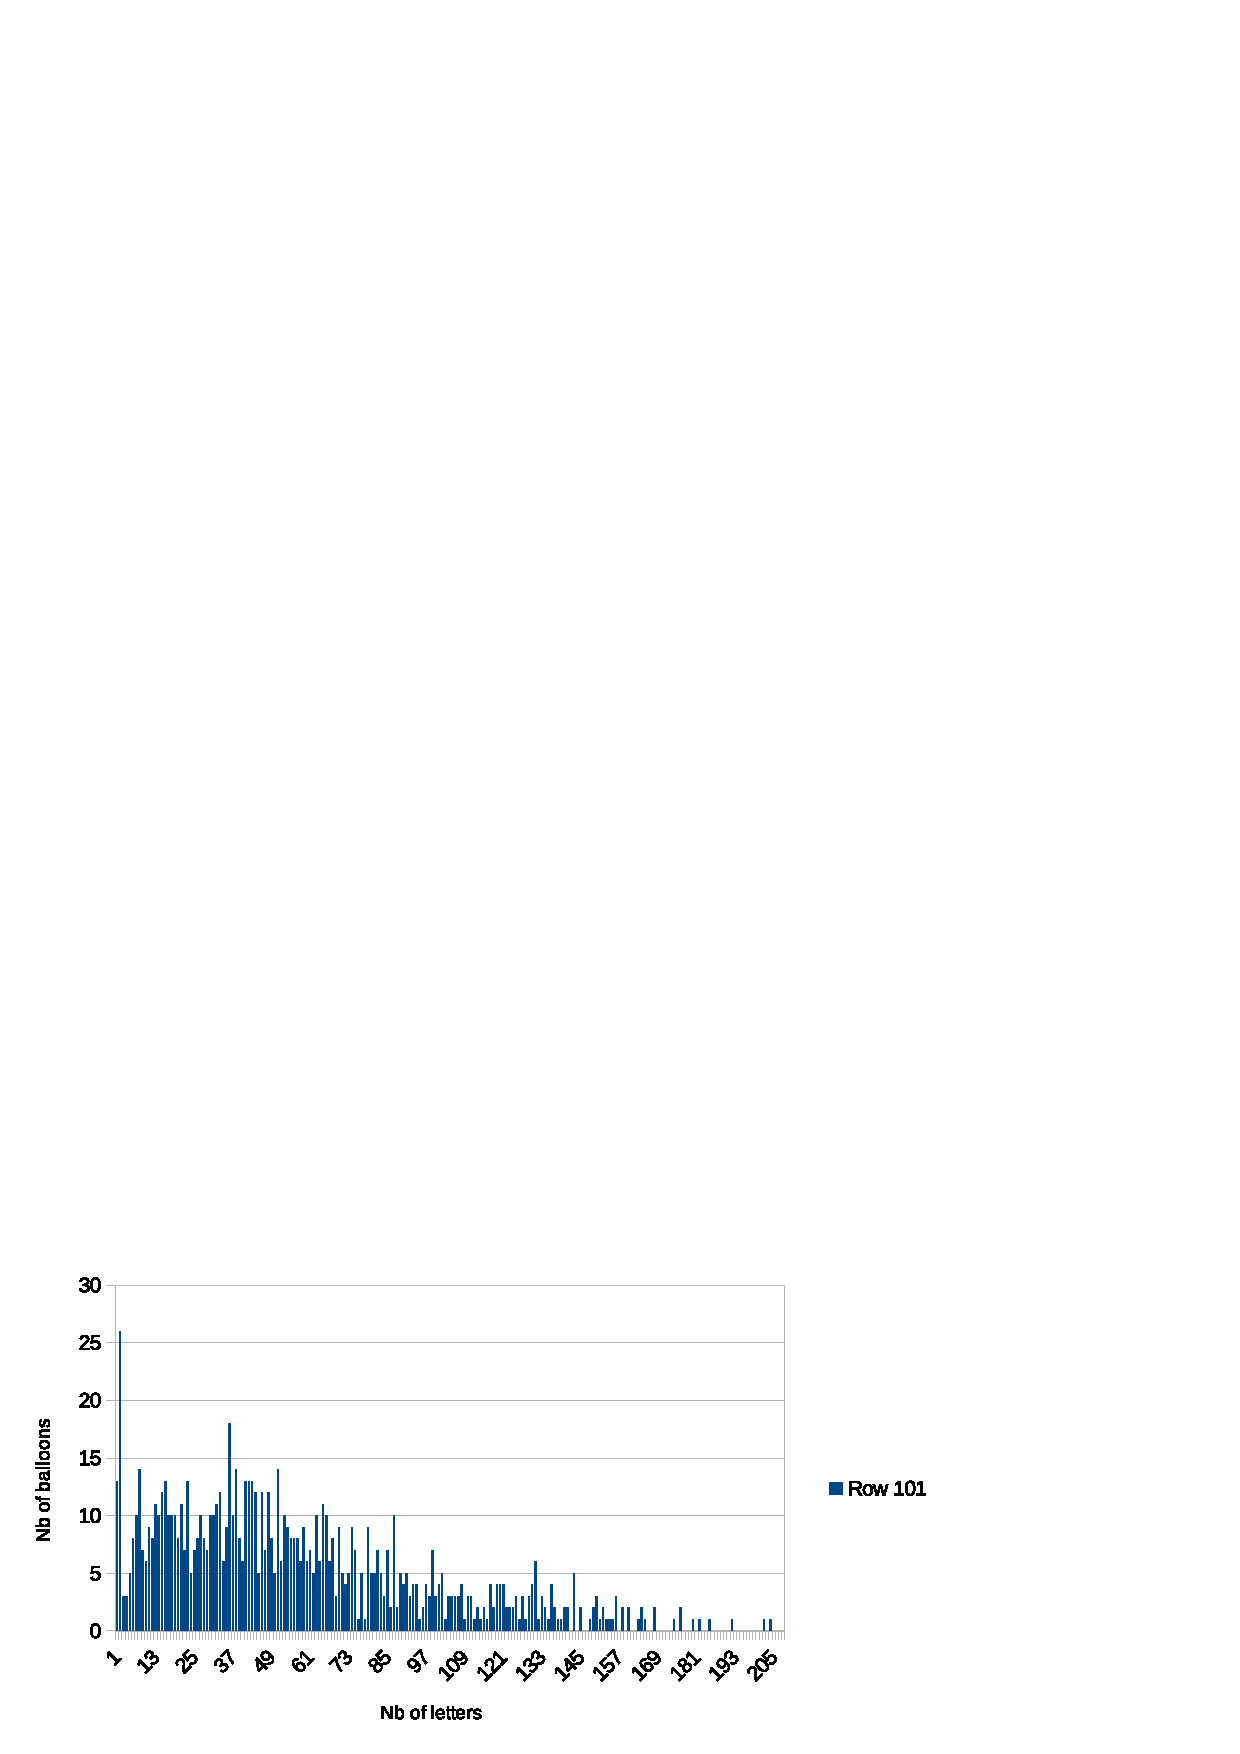
\includegraphics[trim= 10px 0px 60px 0px, clip, width=0.75\textwidth]{number_of_letter_per_balloon.pdf}
      \caption[Distribution of the number of letter per speech balloon]{Distribution of the number of letter per speech balloon.
      }
      \label{fig:ex:min_number_children_validation}
    \end{figure}  
    %%%%%%%%%%%%%%%%%%%%%%%%%%%%%%%%%%%%%%%%%%%%%%%%%%%%%%%%


Note that in Figure~\ref{fig:ex:min_number_children_validation}, there are about 3.5\% of the balloons bellow the selected threshold that contain one or two letters, usually punctuation marks.
%such as ``?'' or ``!''. 
We voluntary omitted them here to avoid detecting a lot of non balloon regions.

Balloons with a confidence value $C_{balloon}$ lower than 10\% were rejected according to the validation experiments on the eBDtheque dataset~\cite{Guerin2013}.
 % table~\ref{tab:balloon_confidence_validation}.

Table~\ref{tab:balloon} shows the average results for the one hundred images of the dataset.
We also compare to a state of the art method from the literature~\cite{Arai11} and our previous work~\cite{rigaud2013active} based on the best results we had obtained for text localisation (Table~\ref{tab:text_results}).


    %%%%%%%%%%%%%%%%%%%%%%%%%%%%%%%%%%%%%%%%%%%%%%%%%%%
  \begin{table}[ht]
    \normalsize
%\renewcommand{\arraystretch}{1.2}

    \centering
    \caption{Balloon extraction results.}
    \begin{tabular}{|c|c|c|c|}
          % \hline
          %   & \multicolumn{2}{|c|}{Character 1}   & \multicolumn{2}{|c|}{Character 2}   \\
          \hline
          &  $R$ (\%)  & $P$ (\%)  & $F$ (\%)   \\
          \hline
          Arai~\cite{Arai11}   & 6.66       & 10.98   & 8.29     \\
          \hline
          %Rigaud~\cite{rigaud2013active} based on GT & 70       & 50     & ?   \\
          Rigaud~\cite{rigaud2013active} & 46.13       & 17.44     & 25.31   \\
          \hline
          Proposed   & 57.90       & 73.84      & 64.91     \\
          \hline
          Proposed + validation  & 54.79       & 88.76      & 67.75     \\
          \hline

          % TOTAL   & 93.4    & 92.8          \\
          % \hline
        %       Proposed multi scale & ???  &???  & ???   & ???       \\
        %   \hline
        \end{tabular}
    \label{tab:balloon}
  \end{table}%
    %%%%%%%%%%%%%%%%%%%%%%%%%%%%%%%%%%%%%%%%%%%%%%%%%%%

%TODO: update Arai's results with is results
%TODO: I can't find the data for Rigaud~\cite{rigaud2013active}, re evaluation is needed

Our method outperforms~\cite{Arai11} thanks to its genericity, since it can process all the image styles of the eBDtheque dataset.
This was expected as~\cite{Arai11} was specifically developed for manga comics that have certain stylistic particularities.
We also surpassed our previous method~\cite{rigaud2013active} because it needs text lines as input which were given in our proposed text extraction method (Section~\ref{sub:text_extraction}).
Here we clearly see the limitations of dependency between the processing.
The performance of our text extractor was 49.75\% (Table~\ref{tab:text_results}) which was used as input for balloon extraction so the balloon extraction~\cite{rigaud2013active} was inevitably affected.
The validation of the expert system once again improve the precision but decreased the recall of the extraction while improving the overall f-measure by almost 3\%.
The drop in recall was due to the balloons that were correctly extracted but which contained no detectable.
%Nevertheless, the proposed method does not beat our previous method~\cite{rigaud2013active} that is also able to extract non closed balloons from text regions (from the ground truth here).
Figure~\ref{fig:text_extraction_detail} confirms that our method works best when the balloons are closed, well segmented and with non cursive text inside.
This experiment was performed in 22 minutes for the whole dataset using one CPU at 2.5GHz (2.2s per balloon on average).



\subsection{Text extraction evaluation} % (fold)
\label{sub:ex:independent_text_extraction_evaluation}
We evaluated our method for text extraction on the 4667 text lines of the eBDtheque dataset~\cite{Guerin2013} ``version 2014'' at object bounding box level.
% according with $th_0=0.5$. % to equation~\ref{eq:recall}.

%We also evaluated the transcription considering as correct the text line with an edit distance $<$ 3 compared to the ground truth.

    %%%%%%%%%%%%%%%%%%%%%%%%%%%%%%%%%%%%%%%%%%%%%%%%%%%
  \begin{table}[ht]
    \normalsize
    \centering
    \caption{Text localisation results.}
    \begin{tabular}{|c|c|c|c|}
          % \hline
          %   & \multicolumn{2}{|c|}{Character 1}   & \multicolumn{2}{|c|}{Character 2}   \\
          \hline
          &  $R$ (\%)  & $P$ (\%)  & $F$ (\%)  \\
          % \hline
          % Before validation   & ?   & ?           \\
          \hline
          Rigaud~\cite{Rigaud2013VISAPP}  & 61.00   & 19.66    & 29.75       \\
          \hline
          Proposed (\cite{Rigaud2013VISAPP}+OCR)  & 60.13   & 42.43   & 49.75        \\
          \hline
          Proposed + validation   & 44.54     & 65.05     & 52.88      \\
          % \hline
          %Proposed (\cite{Rigaud2013VISAPP}+OCR+$ST$ only)  & ?   & ?   & ?        \\
          % \hline
          % Proposed (OCR transcription)  & ?   & ?           \\
          \hline
        \end{tabular}
    \label{tab:text_results}
  \end{table}%
    %%%%%%%%%%%%%%%%%%%%%%%%%%%%%%%%%%%%%%%%%%%%%%%%%%%

In our previous work~\cite{Rigaud2013VISAPP} text extraction was evaluated on a subset of 20 pages of the eBDtheque dataset~\cite{Guerin2013}.
Here we applied it to the whole dataset.
We used our previous method as a baseline to show an improvement in the precision of 20\% when using an OCR-based filter, without a significant loss in recall.
The validation by the expert system improved the precision as expected but also resulted in a drop in recall.
The drop in recall can be explained by the fact that the text extractor is also able to detect texts which are not in the speech balloons but the model considers them as noise.
% in recall that could probably be filled for specific writing style by training the OCR on a specific font. %, when using an OCR system to filter out non text regions.
As in~\cite{Rigaud2013VISAPP}, this method has some difficulty coping with certain types of text that can be found in the comics e.g. graphic sounds.

\paragraph{Text recognition evaluation} % (fold)
\label{par:ex:text_recognition_evaluation}

We also evaluated text transcription using string edit distance~\cite{wagner1974string} between a predicted text transcription given by the OCR and its corresponding transcription in the ground truth. % $T_{gr}$.
The eBDtheque dataset is composed of English, Japanese and French texts.
We evaluated the subset of English and French pages using the OCR with the corresponding training data\footnote{\url{https://code.google.com/p/tesseract-ocr/downloads/list}}. % corresponding to the language defined in the ground truth of each image of the dataset.
This was performed at the text line level taking as correct the text lines that were transcribed exactly as the ground truth transcription, considering all the letters as lower case and ignoring accents (for predicted and ground truth regions).
% with a edit distance $<$ 10\% of their length using equation~\ref{eq:recall} and~\ref{eq:precision}.
%For instance a recognised text line of ten elements will be considered as correct if less than three are split, deleted, transposed, replaced or inserted. 
We obtained a score of $A_{textReco}=$7.18\% which constitute a baseline for future work on text recognition on the eBDtheque dataset~\cite{Guerin2013}.
We performed a more relaxed evaluation where we also considered as correct the text lines at a text edit distance equal to one, the accuracy rise to 10.46\%.
%The distribution of the text line lengths is given in Figure~\ref{fig:textline_lenth_distribution}.
Note that the average text line length is quite short in comic books compared to other documents, the distribution is given Figure~\ref{fig:ex:textline_lenth_distribution} for the eBDtheque dataset.

    %%%%%%%%%%%%%%%%%%%%%%%%%%%%%%%%%%%%%%%%%%%%%%%%%%%%%%%%
    % \begin{figure}[ht]%trim=l b r t  width=0.5\textwidth,  
    %   \centering
    %   \includegraphics[trim= 0px 5px 65px 5px, clip, width=0.85\textwidth]{number_of_letter_per_textline.png}
    %   \caption[Distribution of the number of letter per text lines]{Distribution of the number of letter per text lines.
    %   }
    %   \label{fig:textline_lenth_distribution}
    % \end{figure}  
    %%%%%%%%%%%%%%%%%%%%%%%%%%%%%%%%%%%%%%%%%%%%%%%%%%%%%%%%

% Note that in Figure~\ref{fig:ex:textline_lenth_distribution}, there are more than a hundred text lines of only one letter corresponding to punctuation or single letter words such as ``I'' or ``A''; this is a particularity of comics.

% paragraph text_recognition_evaluation (end)


\subsection{Comic character extraction evaluation} % (fold)
\label{ssub:independent_comic_character_extraction_evaluation}

We evaluated our method for character spotting on \modif{??} of 1550 comic character instances of the eBDtheque dataset~\cite{Guerin2013} ``version 2014'' at object bounding box level.

To perform this experiments, we asked the users to manually highlight the object position as described in section~\ref{sec:input_query}.
The selection usually includes hair, head and top body colours because lower body parts are often hidden by the frame border or the posture. 
From the user pixel selection, we computed the bounding box to show that the system does not need a precise object colour selection. 
We reduced the number of colour to a \modif{standard web palette $P_c$ of 256 colours} because comics are colourful drawings similar to web pages and icons that contain a limited number of colour. 
We fixed the descriptor size to $N=3$ according to the evaluation figure~\ref{fig:ex:descriptor_size_evaluation}.
In the retrieval process, we set $T=N$ which means that the confidence of the candidate region equal 100\% (all the query colours must be present in the candidate region to be considered as a correct detection).
We used three squared window sizes according to the query height: half of the query height, query height and twice the query height.


%%%%%%%%%%%%%%%%%%%%%%%%%%%%%%%%%%%%%%%%%%%%%%%%%%%
 \begin{figure}[!ht]  %trim=l b r t  width=0.5\textwidth,
   \centering
  \includegraphics[trim= 5mm 0mm 30mm 0mm, clip, width=250px]{descriptor_size_evaluation.png}
  \caption[Character spotting descriptor size validation]{Descriptor size validation. Measure of recall (blue square) and precision (red diamond) detection for different descriptor sizes from a testing set of 17 comics pages. The maximum recall is for $N=3$.}
  \label{fig:ex:descriptor_size_evaluation}
 \end{figure}
%%%%%%%%%%%%%%%%%%%%%%%%%%%%%%%%%%%%%%%%%%%%%%%%%%%


\paragraph{Performance evaluation}
The following results were obtained with the common evaluation measures of recall, precision at object level which means that we considered as correctly detected the objects that are overlapped by a detected region without considering the percentage of overlapping.
Recall ($R$) is the number of correctly detected object divided by the number of objects to detect.
Precision ($P$) is the number of correctly detected objects divided by the number of detected objects.
%Each detected object $D$ was compared to the corresponding ground truth one $G$ with the nearest centroid, considering only one matching per ground truth balloon.
We consider as candidate regions, regions that have $C=100\%$ confidence (contains at least all the descriptor colours).% Lower confidence detection need additional processing to be considerate as correct results.

We evaluated our method on 34 comics pages from 10 different albums which represent 22 comic characters that appear 352 times in total. We obtained 90.3\% recall and 46.7\% precision in average. Results are detailed in table~\ref{tab:ex:character_spotting_detail_result} where album 1 to 10 correspond to MIDAM GAMEOVER T05, TARZAN COCHON, CYB COSMOZONE, CYB MAGICIENLOOSE, CYB MOUETTEMAN, LAMISSEB LESNOEILS1, LUBBIN LESBULLESDULABO, MIDAM KIDPADDLE7, PIKE BOYLOVEGIRLS T41 and TRONDHEIM LES TROIS CHEMINS 005 respectively from the eBDtheque dataset~\cite{Guerin2013}. %Another album of two pages has also been evaluated, we had 83\% recall and 66\% precision score.


\begin{table}[htbp]
\caption{Character detection performance}
\begin{tabular}{|c|l|l|r|r|r|}
\hline
\multicolumn{1}{|c|}{\textbf{Album}} & \multicolumn{1}{c|}{\textbf{Nb pages}} & \multicolumn{1}{c|}{\textbf{Nb character}} & \multicolumn{1}{c|}{\textbf{Character ID}}  & \multicolumn{1}{c|}{\textbf{Recall}} & \multicolumn{1}{c|}{\textbf{Precision}} \\ \hline
\multicolumn{1}{|r|}{1}  & \multicolumn{1}{r|}{10} & \multicolumn{1}{r|}{2} & 0  & 92.3\% & 16.8\% \\ \hline
 &  &   & 1 & 91.8\% & 65.0\% \\ \hline
\multicolumn{1}{|r|}{2}  & \multicolumn{1}{r|}{1} & \multicolumn{1}{r|}{1} & 2  & 75.0\% & 26.5\% \\ \hline
\multicolumn{1}{|r|}{3}  & \multicolumn{1}{r|}{5} & \multicolumn{1}{r|}{4} & 3  & 100.0\% & 50.0\% \\ \hline
 &  &   & 4  & 93.3\% & 60.9\% \\ \hline
 &  &   & 5  & 100.0\% & 33.3\% \\ \hline
 &  &   & 6  & 100.0\% & 100.0\% \\ \hline
\multicolumn{1}{|r|}{4}  & \multicolumn{1}{r|}{1} & \multicolumn{1}{r|}{1} & 7  & 85.7\% & 85.7\% \\ \hline
\multicolumn{1}{|r|}{5}  & \multicolumn{1}{r|}{4} & \multicolumn{1}{r|}{2} & 8 & 100.0\% & 75.0\% \\ \hline
 &   &  & 9 & 50.0\% & 27.8\% \\ \hline
\multicolumn{1}{|r|}{6}  & \multicolumn{1}{r|}{5} & \multicolumn{1}{r|}{2} & 10 & 71.8\% & 10.1\% \\ \hline
 &   &  & 11  & 100.0\% & 29.9\% \\ \hline
\multicolumn{1}{|r|}{7}  & \multicolumn{1}{r|}{2} & \multicolumn{1}{r|}{2} & 12 & 100.0\% & 13.8\% \\ \hline
 &   &  & 13 & 100.0\%  & 54.5\% \\ \hline
 &   &  & 14 & 100.0\%  & 55.6\% \\ \hline
\multicolumn{1}{|r|}{8}  & \multicolumn{1}{r|}{2} & \multicolumn{1}{r|}{2} & 15 & 81.8\% & 75.0\% \\ \hline
 &   &  & 16 & 100.0\%  & 12.7\% \\ \hline
\multicolumn{1}{|r|}{9}  & \multicolumn{1}{r|}{2} & \multicolumn{1}{r|}{1} & 17 & 83.3\% & 58.8\% \\ \hline
\multicolumn{1}{|r|}{10} & \multicolumn{1}{r|}{2} & \multicolumn{1}{r|}{4} & 18 & 81.3\% & 35.1\% \\ \hline
 &   &  & 19 & 100.0\% & 48.4\% \\ \hline
 &   &  & 20 & 92.9\% & 17.1\% \\ \hline
 &   &  & 21 & 90.9\% & 24.4\% \\ \hline
 %&  &  &  & \multicolumn{1}{l|}{} & \multicolumn{1}{l|}{} & \multicolumn{1}{l|}{} & \multicolumn{1}{l|}{} & \multicolumn{1}{l|}{} & \multicolumn{1}{l|}{} & \multicolumn{1}{l|}{} \\ \hline
 &  &  &  & &  \\ \hline %\multicolumn{1}{l|}{} & \multicolumn{1}{l|}{} & \multicolumn{1}{l|}{} & \multicolumn{1}{l|}{} & \multicolumn{1}{l|}{} & \multicolumn{1}{l|}{} & \multicolumn{1}{l|}{} \\ \hline
\multicolumn{1}{|r|}{\textbf{10}} & \multicolumn{1}{r|}{\textbf{34}} & \multicolumn{1}{r|}{\textbf{22}} & \multicolumn{1}{r|}{\textbf{22}} & \textbf{90.3\%} & \textbf{46.7\%} \\ \hline
\end{tabular}
\label{tab:ex:character_spotting_detail_result}
\end{table}


\paragraph{Detection results}
% \label{sec:eval}

We evaluated present interesting detection results based on a three colours user defined query descriptor (see section~\ref{sec:proposed_method}). 
The processing time was about 6 seconds per image for a A4 300DPI image on a regular machine. Most of the time consumption is for the mask creation and it is proportional to the number of mask to create.  Detection result examples are presented figure~\ref{fig:ex:character_spotting_results}.

The detected region aims to localize the smallest regions containing all the colours of the query descriptor. This region is usually smaller than the ground truth region which is defined at character bounding box level. A post processing is needed to compute the character bounding box from the detected region by extending it to the colour region boundaries.

%%%%%%%%%%%%%%%%%%%%%%%%%%%%%%%%%%%%%%%%%%%%%%%%%%%
 \begin{figure}[!ht]  %trim=l b r t  width=0.5\textwidth,
   \centering
  \includegraphics[width=0.5\textwidth]{result_exemples.png}
  \caption[Character spotting result sample]{
  Each line shows a character query region bounding box in white (left column), a correct detection (middle column) and a wrong detection (right column). Green rectangles represents the ground truth region and the red rectangle corresponds to the region detections. The corresponding character IDs in table~\ref{tab:ex:character_spotting_detail_result} are 12, 8, 0, 10, 16 and 2 from top to bottom. %and second columns show correct and wrong detection result for album 1. Third and fourth columns are correct and wrong detection results examples from album 2. Top first and top third columns are the user defined queries. %{\bf Update true and false positive examples and draw detection window (according to $S$ definition)
  }
  \label{fig:ex:character_spotting_results}
 \end{figure}
%%%%%%%%%%%%%%%%%%%%%%%%%%%%%%%%%%%%%%%%%%%%%%%%%%%

Correct detections show the variety of comics character position and deformation that we are able to detect with the presented framework. There are few missing detection and over detection are essentially due to other comics character detection and image pre processing (colour reduction).%character part missing, small size objects or low resolution images.

    %%%%%%%%%%%%%%%%%%%%%%%%%%%%%%%%%%%%%%%%%%%%%%%%%%%
%   \begin{table}[ht]
%     \normalsize
% \renewcommand{\arraystretch}{1.2}
% 
%     \centering
%     \caption{Comics character detection results.}
%     \begin{tabular}{|c|c|c|c|c|}
%           \hline
%             & \multicolumn{2}{|c|}{Character 1}   & \multicolumn{2}{|c|}{Character 2}   \\
%           \hline
%           &  Detected   & Missed    &  Detected  & Missed   \\
%           \hline
%           Album 1, p. 1   & 7       & 2     & 95.9      & 90.1    \\
%           \hline
%           Album 1, p. 2   & 8       & 2     & 78.4      & 94.8    \\
%           \hline
%           Album 1, p. 3   & 5   & 1     & 97.7    & 88.7      \\
%           \hline
%           TOTAL   & 93.4    & 92.8    & 97.7    & 88.7      \\
%           \hline
%         %       Proposed multi scale & ???  &???  & ???   & ???       \\
%         %   \hline
%         \end{tabular}
%     \label{tab:high_res}
%   \end{table}%
    %%%%%%%%%%%%%%%%%%%%%%%%%%%%%%%%%%%%%%%%%%%%%%%%%%%



%balloon localization performance at bounding box level to highlight the benefits of both active contour theory and domain specific knowledge. Second, we performed pixel level evaluation on a smaller subset to show the ability of our method to fit balloon contour details.


\paragraph{Discussion}
The proposed framework gives promising results for contemporary comics, we also tried on historical such as FRED PHILEMON12 and MCCALL ROBINHOOD from the eBDtheque dataset but the printing process generates a lot of noise (thickness of ink). 
A pre-processing smoothing~\cite{l0smoothing2011} is required in this case. The colour palette we used has 256 colours, we believe that we can improve the presented method by computing the palette from the user's query in order to ignore unwanted colours and speed up the process. 
The sliding windows approach does not allow to segment comics character at a pixel level, a distance measure between the colour mask regions could solve this.
 Also, once we retrieved all colour similar objects, we could learn a shape model and try to find more objects occurrences based on shape information in a second stage, this will be a future work.


% ssubsection independent_comic_character_extraction_evaluation (end)

% subsection independent_information_extraction_evaluation (end)
\section{Knowledge-driven analysis evaluation} % (fold) %IJDAR
\label{sub:ex:knowledge_driven_analysis_evaluation}


%-------------------------------------------------------------------------
% \subsection{Framework evaluation}
We evaluated our framework during the two iterations of the process loop introduced in Chapter~\ref{chap:knowledge} and particularly at the beginning (Step 1: hypothesis) and at the end (Step 3: inference) of each iteration.
Note that using this framework some processes ($C$, $STSB$, $SBCS$) were related to previous processes which propagated errors and reduced their performance compared to their separated evaluation in Section~\ref{sub:ex:independent_information_extraction_evaluation}.

We evaluate our framework using the f-measure of panel $P$, balloon $B$, text $T$ and character $C$ extractions.
Also, the accuracy of the two semantic links $STSB$ and $SBSC$ is measured.
%  are all automatic here with their respective error rates. panel $P$, balloon $B$ and text $T$ extraction are similar to the 
The change in the amount of information discovered throughout the process is presented in Figure~\ref{fig:ex:score_evolution}.% were we show the % are evaluated using .

TODO ADD TABLE WITH NUMBERS CORREPONDING TO RADAR CHARTS


% \begin{figure}[ht!]
% \centering
% \begin{subfigure}[b]{115px}
% \includegraphics[width=115px]{fig/radar_a.png}
% \caption{Hypothesis}
% \label{fig:ex:score_evolution_a}
% \end{subfigure}
% \begin{subfigure}[b]{115px}
% \includegraphics[width=115px]{fig/radar_b.png}
% \caption{Validation \& inference}
% \label{fig:ex:score_evolution_b}
% \end{subfigure}
% \begin{subfigure}[b]{115px}
% \includegraphics[width=115px]{fig/radar_c.png}
% \caption{Hypothesis}
% \label{fig:ex:score_evolution_c}
% \end{subfigure}
% \begin{subfigure}[b]{115px}
% \includegraphics[width=115px]{fig/radar_d.png}
% \caption{Validation \& inference}
% \label{fig:ex:score_evolution_d}
% \end{subfigure}
% \caption{Performance evolution for panels $P$, balloons $B$, text lines $T$, comic characters $C$ and the semantic links $STSB$ and $SBSC$ at the hypothesis and evaluation steps during the two loops of the proposed process.
%   The dashed blue line represents the best score using the proposed model on the data extracted from the ground truth data (optimal condition).
%   The solid red line is the performance of the framework using all the automatic extractions and semantic link inferences presented in this paper.}

%   \label{fig:ex:score_evolution}
% \end{figure}


%%%%%%%%%%%%%%%%%%%%%%%%%%%%%%%%%%%%%%%%%%%%%%%%%%%
\begin{figure}[ht]  %trim=l b r t  width=0.5\textwidth,
  \centering
 \includegraphics[width=230px]{radar_chart.png}
 \caption[Knowledge-driven extraction performance evolution]{Change in performance for panels $P$, balloons $B$, text lines $T$, comic characters $C$ and the semantic links $STSB$ and $SBSC$ at the hypothesis and evaluation steps during the two loops of the process.
 The dashed blue line represents the best score using our model on the data extracted from the ground truth data (optimal condition).
 The solid red line is the performance of the framework using all the automatic extractions and semantic link inferences presented in this paper.}
 \label{fig:ex:score_evolution}
\end{figure}
%%%%%%%%%%%%%%%%%%%%%%%%%%%%%%%%%%%%%%%%%%%%%%%%%%%

%TODO: add tail results figure + legend + analysis
\paragraph{Process details} % (fold)
\label{par:process_details}

% paragraph process_details (end)
Figure~\ref{fig:ex:score_evolution} shows the change of the performance of our framework after the first and second iteration of analysis over the eBDtheque dataset~\cite{Guerin2013}.
The performance of the first iteration was measured after the initial extraction of simple elements which were considered as hypotheses by the expert system (Figure~\ref{fig:ex:score_evolution}a.) and after validation by the expert system (Figure~\ref{fig:ex:score_evolution}b.).
Between the first initialization and validation (first row of Figure~\ref{fig:ex:score_evolution}), the f-measure remained stable for $P$ and increased by 3\% for the balloon $B$ and text $T$.
% which reflects the first contribution of the expert system over the low level processing.
%In fact, the text extraction has a 49\% precision (see table~\ref{tab:text_results}) which is raised up to 72\% by using the rule-based contextual filtering but this has also a cost for the recall which is dropped by 23\%. 
% into more specific elements such as speech balloon $SB$ and speech text $ST$ in order to provide additional information to the second iteration.
At this point, no comic book characters were discovered because their rules in the ontology are related to elements that were not yet discovered.
Nevertheless, the semantic links between speech text and balloon $STSB$ were inferred (47.6\%).
The expert system applied the inference rules to automatically label the balloon with a tail that included text such as speech balloon $SB$ and speech text $ST$ respectively and created a semantic link $STSB$ between each of them.

The newly inferred links were processed by the expert system along with previously validated regions during a second iteration in order to get more information by trying to apply more rules from the knowledge base.
This time, the expert system could make use of rules related to characters because the speech balloons were now part of the knowledge base.
Panels and speech balloons were used to create hypotheses for the location of characters and then the low level processing located them more precisely within these regions (Figure~\ref{fig:ex:score_evolution}c.).
Finally, the expert system validated the newly discovered regions and inferred the semantic links between speech balloons and speaking characters $SBSC$ (Figure~\ref{fig:ex:score_evolution}d.).

% \modifc{ADD Clement: results analysis to explain (and illustrate with examples?) why the results on data from the ground truth are not perfect.}

% In figure~\ref{fig:ex:score_evolution}, the dashed blue line represents how fit the model to the dataset according to section~\ref{sub:knowledge_base} and therefore sets the maximum reachable score for each of the elements using the presented framework on this data.

\paragraph{Low level processing} % (fold)
\label{par:low_level_processing}

% paragraph low_level_processing (end)
The low level processing scores ($P$, $B$, $T$) always increased between the hypothesis and the validation steps, which confirms the benefits of combining different levels of analysis.
The best extraction performance was obtained for the panels that were usually the easiest elements to extract from a page.
% because they overlap most of the content.
The lowest extraction performance was for the comic characters $C$.
% First, the non-extraction of comic characters that do not speak, second the difficulty of locating precisely comics characters in all the different comics styles that compose the eBDtheque dataset 
There are various reasons for this.
First, the limitation of the extractor to process speaking characters; second, the variability of character styles in the eBDtheque dataset; third, the error propagation of previous processes (panel, text, balloon, tail and semantic link extractions) that are required to guess comic character locations.

%, they represent more than half of them.

\paragraph{Semantic links} % (fold)
\label{par:global_semantic_links}

%We evaluated the ability of our system to produce the semantic relations introduced in \ref{sub:knowledge_base}, namely \textit{STSB} and \textit{SBSC}, based on the correctly extracted balloons (see section~\ref{sub:balloon_evaluation}) and  text lines (see section~\ref{sub:text_localisation_recognition_evaluation}).
The expert system was able to retrieve 47.6\% of the $STSB$ and 18\% of the $SBSC$ relations, which represents more than 25\% of what could possibly be detected using the proposed model.

It should be stressed that these numbers represent the efficiency of the last process of the whole framework pipeline.
Individual errors at each recognition and validation step of the pipeline are propagated to the final semantic association between elements ($SBSC$).
Therefore a single improvement in the detection or the validation of any kind of element would have an impact at the semantic association level.


\paragraph{General evaluation} % (fold)
\label{par:global_evaluation}
It is difficult to combine individual metrics of a different nature into a single global metric.
As an indicative metric, we considered the hexagon area as being the amount of information that could be retrieved from the eBDtheque dataset~\cite{Guerin2013}.
Our model is theoretically able to model 88.83\% of this information (dashed line), despite the diversity of the images in this dataset, and 54.89\% of this information can be retrieved automatically (solid line) using our framework.




% subsection knowledge_driven_analysis_evaluation (end)

\section{Global evaluation} % (fold)
\label{sub:ex:global_evaluation}

TODO ???

%big table to compare the 3 level of contribution of this thesis

      %                 | sequential|Independent|Knowledge-driven |
      %Panel            | R | P | F | R | P | F |  R  |  P  |  F  |
      %Text             |
      %Balloon          |
      %Tail                   ? 
      %Comic character
      %Semantic link STSB                 X             
      %Semantic link SBSC                 X

% subsection global_evaluation (end)
% section evaluation (end)


% Conclusion --------------------------------------------------------------------------------------------------------------------------------------
\section{Conclusions}
\label{sub:ex:conclusion}

TODO
